\documentclass[11pt]{article}
\usepackage[T1]{fontenc}
\usepackage[utf8]{inputenc}
\usepackage{lmodern}
\usepackage[margin=1in]{geometry}
\usepackage{amsmath,amssymb,amsthm,mathtools}
\usepackage{microtype}
\def\DoNotLoadEpstopdf{}
\usepackage{tikz}
\usetikzlibrary{arrows.meta,calc,patterns}
\usepackage{xcolor}
\usepackage[colorlinks=true,linkcolor=blue!45!black,citecolor=blue!45!black,urlcolor=blue!45!black]{hyperref}
\usepackage{bookmark}
\hypersetup{pdftitle={Nearly minimal maxima and positive minima of Littlewood polynomials},pdfauthor={OpenAI}}
\newtheorem{theorem}{Theorem}[section]
\newtheorem{proposition}[theorem]{Proposition}
\newtheorem{lemma}[theorem]{Lemma}
\newtheorem{corollary}[theorem]{Corollary}
\theoremstyle{definition}
\newtheorem{definition}[theorem]{Definition}
\theoremstyle{remark}
\newtheorem{remark}[theorem]{Remark}
\newcommand{\T}{\mathbb T}
\newcommand{\R}{\mathbb R}
\newcommand{\Z}{\mathbb Z}
\newcommand{\N}{\mathbb N}
\newcommand{\C}{\mathbb C}
\newcommand{\e}{\mathrm e}
\newcommand{\norm}[1]{\left\lVert #1\right\rVert}
\DeclareMathOperator{\sgn}{sgn}
\title{Nearly minimal maxima and positive minima\\of Littlewood polynomials}
\author{OpenAI}
\date{October 5, 2026}
\begin{document}
\maketitle
\begin{abstract}
For every $\eta>0$ and every sufficiently large integer $N$, there is
a polynomial with $N$ consecutive coefficients in $\{-1,1\}$ whose modulus
lies between $\sqrt N/16$ and $(1+\eta)\sqrt N$ everywhere on the unit
circle.
\end{abstract}
\tableofcontents
\section{Introduction}\label{sec:introduction}
A \emph{Littlewood polynomial of length $N$} is a polynomial
\[
 P(z)=\sum_{k=0}^{N-1}\varepsilon_kz^k,
 \qquad \varepsilon_k\in\{-1,1\}.
\]
Write $\T=\R/\Z$ and $\e(t)=\exp(2\pi i t)$, and give $\T$ probability
Haar measure. Parseval's identity gives
\[
 \int_{\T}|P(\e(t))|^2\,dt=N,
 \qquad
 \norm{P}_\infty:=\max_{t\in\T}|P(\e(t))|\ge\sqrt N.
\]
We ask whether a maximum arbitrarily close to this lower bound can
coexist with a minimum bounded below by a fixed positive multiple of
$\sqrt N$.

\begin{theorem}\label{thm:main}
For every $\eta>0$ there is an integer $N_0=N_0(\eta)$ such that, for every
integer $N\ge N_0$, there exist real signs
$\varepsilon_0,\ldots,\varepsilon_{N-1}$ for which
\[
 \frac1{16}\sqrt N
 \le\left|\sum_{k=0}^{N-1}\varepsilon_kz^k\right|
 \le(1+\eta)\sqrt N
 \qquad (|z|=1).
\]
\end{theorem}

The lower constant is independent of the accuracy of the upper bound.
The conclusion holds for a single polynomial at every sufficiently large
length, on the entire circle, including the real points $1$ and $-1$.

\subsection{Context and antecedents}
Questions about the flatness of polynomials with restricted coefficients
have a long history in harmonic analysis. The two-sided flatness question
appears in Erd\H{o}s's problems \cite[Problem 26]{Erdos1957} and in
Littlewood's work \cite{Littlewood1966}. The Rudin--Shapiro construction
of real-sign polynomials gives an upper bound $\sqrt{2N}$ at dyadic lengths
\cite{Rudin1959}. The requirement that the coefficients be real signs is
substantial: Kahane constructed polynomials with complex unimodular
coefficients whose normalized modulus tends uniformly to one
\cite{Kahane1980}; see also Bombieri and Bourgain
\cite{BombieriBourgain2009}. The real-sign questions and their relation to
the Parseval lower bound are discussed in
\cite[Problems 4.13 and 4.31]{HaymanLingham2018}.

Balister, Bollob\'as, Morris, Sahasrabudhe and Tiba proved that flat
Littlewood polynomials exist at every degree at least two: their modulus lies between
two absolute positive multiples of the square root of the length
\cite[Theorem 1.1]{BalisterEtAl2020}. The companion manuscript
\cite{OpenAIMinimal} establishes that the best possible upper constant
tends to one through all lengths. Theorem~\ref{thm:main} combines the
nearly minimal upper bound with a fixed positive lower bound. These two
properties must be achieved by the same choice of signs, so neither of the
preceding existence statements supplies the conclusion by itself.

The construction in \cite{OpenAIMinimal} provides more than an upper bound.
It gives relaxed real coefficients in $[-1,1]$ whose Fourier polynomial
is uniformly approximated by quadratic-phase waves with disjoint supports.
The modulus of this leading term has almost full mean-square mass, but it vanishes
on some arcs. We reproduce the auxiliary polynomial, interval packing,
sampling, and rounding arguments needed here. The standard external
inputs are the Pippenger--Spencer hypergraph-coloring theorem and the
Lovett--Meka partial-coloring theorem, stated at their points of use.

Our additional step constructs a correction on the arcs where the leading
amplitude is small. On each arc its phase is $N$ times a fixed piecewise
quadratic function, plus an affine adjustment with slope bounded
independently of $N$. We call the fixed function the leading phase.
At a transition, the correction and existing wave have the same leading
phase derivative, and the affine adjustment makes their full phase values
agree modulo integers. This keeps the waves aligned while the correction turns on.
Across most of each arc, the leading phase derivative runs through an
interval assigned only to that arc and its reflection. This separation controls individual
Fourier coefficients; keeping that derivative strictly between zero and
one controls the Fourier mass
outside the permitted degrees. The two estimates preserve both the
coefficient constraint and a lower-modulus margin.

The proof of \cite{BalisterEtAl2020} also repairs small-modulus regions:
a cosine polynomial from the Rudin--Shapiro construction is supplemented
by a sine polynomial that is large on the exceptional arcs, with
discrepancy estimates controlling the coefficients. Here the correction
acts on the quadratic waves of \cite{OpenAIMinimal}, and its coefficient
cost tends to zero as the upper bound approaches its minimum.

\subsection{Proof strategy and notation}
For a real vector $X=(X_0,\ldots,X_{N-1})$, write
\[
 U_X(t)=\frac1{\sqrt N}\sum_{k=0}^{N-1}X_k\e(kt),
 \qquad
 \mu(X)=\frac12\sum_{k=0}^{N-1}(1-|X_k|)
 \quad\text{if }X\in[-1,1]^N.
\]
The quantity $\mu(X)$ measures how far the coefficients are from signs.
The rounding estimate proved in Section~\ref{sec:rounding} changes $U_X$
by at most
\[
 \frac C{\sqrt N}
 +C\sqrt{\frac{\mu(X)}N
          \log\!\left(\frac{80N}{\mu(X)}\right)},
\]
with the square-root term defined to be zero at $\mu(X)=0$.
Thus a small relative defect permits a uniformly small change on the whole
circle. The construction must create its positive lower bound before this
rounding is applied.

Fix a small accuracy parameter $\delta>0$. Sections~\ref{sec:spreading}
and~\ref{sec:packing} construct a bounded real trigonometric polynomial
on an auxiliary torus and pack the angle intervals that will support
the resulting quadratic waves. Section~\ref{sec:sampling} produces vectors $Y_N\in[-1,1]^N$ and
leading functions $B_N$ with
\[
 U_{Y_N}=B_N+o(1),\qquad |B_N|=B\le1+O(\delta),\qquad
 \int_{\T}B^2\ge1-O(\delta).
\]
Here $B$ is a fixed sum of disjoint smooth bumps, independent of
$N$. In particular, the arcs where $B<1/8$ have total length $O(\delta)$.

Section~\ref{sec:correction} constructs a conjugate-symmetric function
$R_N$ on those arcs such that $B_N+R_N$ has minimum at least $1/8-o(1)$,
without raising its maximum. The essential Fourier estimates are
\[
 \sqrt N\,|\widehat R_N(k)|=O(\sqrt\delta)\quad(0\le k<N),
 \qquad
 \sum_{k\notin\{0,\ldots,N-1\}}|\widehat R_N(k)|=o(1).
\]
The first bound permits a small rescaling that returns the corrected real
coefficients to $[-1,1]$. The second shows that restricting the correction
to the required degrees preserves its uniform effect on the circle.
The rescaled coefficients still have relative defect tending to zero with
$\delta$. Section~\ref{sec:completion} applies the rounding estimate and
chooses the parameters to prove Theorem~\ref{thm:main}.

All torus integrals below use probability Haar measure. For an integrable
function $f$ on $\T^m$ we use
\[
 \widehat f(a)=\int_{\T^m}f(y)\e(-a\cdot y)\,dy
 \qquad(a\in\Z^m).
\]
All auxiliary dimensions, frequencies, intervals, and smooth cutoffs are
fixed after $\delta$ is chosen. Unless another limit is specified, $o(1)$
denotes a quantity tending to zero as $N\to\infty$ with these data fixed.
Constants denoted by $O_\delta$ may depend on these fixed data.
An \emph{absolute} constant is independent of both $\delta$ and $N$.

\section{Spreading Fourier coefficients}
\label{sec:spreading}

This section supplies the auxiliary polynomial used in the sampling
construction.  We reproduce the coefficient-spreading argument of
\cite[Section~4]{OpenAIMinimal}, constructing a real trigonometric
polynomial with almost unit mean-square mass whose Fourier coefficients
fit within a total spectral width less than one.
The coefficient assigned to a width $w$ must have size at
most approximately $\sqrt w$: this is the normalization of the quadratic
integral in Lemma~\ref{lem:quadratic}.  Additional torus variables let us
distribute each coefficient among many frequencies while controlling
both their number and their sizes.

For a trigonometric polynomial $F$ on $\T^m$, write
\[
 \widehat F(a)=\int_{\T^m}F(x)\e(-a\cdot x)\,dx,
 \qquad a\in\Z^m.
\]
A finite set is a \emph{containing Fourier support} if every coefficient
outside it vanishes; coefficients inside it are allowed to vanish as well.
All norms and integrals on tori use probability Haar measure.

\begin{proposition}[An auxiliary polynomial with controlled widths]
\label{prop:auxiliary}
For every $0<\delta<1/20$, there exist integers $m\ge1$ and $r\ge2$,
nonzero vectors $a_1,\ldots,a_r\in\Z^m$, a real-valued trigonometric
polynomial $F$ on $\T^m$, and a vector $v\in\R^m$ with the following
properties.  No two of the vectors $a_i$ are parallel, and
\[
 \mathcal A=\{a_1,-a_1,\ldots,a_r,-a_r\}
\]
is a containing Fourier support of $F$.  Moreover,
\begin{equation}
 \label{eq:auxiliary-norms}
 \norm{F}_\infty\le1,
 \qquad \norm{F}_2\ge1-3\delta.
\end{equation}
Writing $\lambda_a=a\cdot v$ for $a\in\mathcal A$, we have
\begin{equation}
 \label{eq:auxiliary-widths}
 \lambda_a\ne0,
 \qquad \sum_{a\in\mathcal A}|\lambda_a|<1,
 \qquad
 \frac{|\widehat F(a)|}{\sqrt{|\lambda_a|}}
 \le K_\delta,
 \qquad
 K_\delta=\sqrt{\frac{(1+\delta)^3}{1-\delta}}.
\end{equation}
All these objects depend on $\delta$ alone.
\end{proposition}

The construction starts with a polynomial of almost unit mean square.
Quadratic oscillations in new variables spread its coefficients; finite
Fourier truncation then gives the required polynomial.  We first record
the uniform quadratic estimate used to control the spread coefficients.

\begin{lemma}[Uniform quadratic integration]
\label{lem:quadratic}
Let $g\in C_c^\infty(\R)$ and let $\beta\in\R\setminus\{0\}$ be fixed.
As $T\to\infty$ through positive real values,
\begin{equation}
 \label{eq:uniform-quadratic}
 \begin{split}
 \int_{\R}g(x)\e(T\beta x^2/2-ux)\,dx
 ={}&\frac{\e(\operatorname{sgn}(\beta)/8-u^2/(2T\beta))}
 {\sqrt{T|\beta|}}\\
 &\qquad\cdot\left(g\left(\frac{u}{T\beta}\right)
       +O_{g,\beta}(T^{-1})\right),
 \end{split}
\end{equation}
uniformly for every real $u$.
\end{lemma}

\begin{proof}
Use the real-line Fourier transform
$\widehat g(\xi)=\int_{\R}g(x)\e(-\xi x)\,dx$, and put
$x_0=u/(T\beta)$.  Completing the square reduces the integral to
\[
 \e\left(-\frac{u^2}{2T\beta}\right)
 \int_{\R}g(x_0+y)\e(T\beta y^2/2)\,dy.
\]
Insert the damping factor $\exp(-\pi\rho y^2)$ with $\rho>0$, and use
Fourier inversion on $g(x_0+y)$.  The resulting double integral is
absolutely integrable.  The inner Gaussian integral is
\[
 \int_{\R}\exp\bigl(-\pi(\rho-iT\beta)y^2+2\pi i\xi y\bigr)\,dy
 =(\rho-iT\beta)^{-1/2}
   \exp\left(-\frac{\pi\xi^2}{\rho-iT\beta}\right).
\]
Here the square root is the branch analytic in the right half-plane
and positive on the positive real axis.  As $\rho\downarrow0$,
\[
 (\rho-iT\beta)^{-1/2}
 \longrightarrow\frac{\e(\operatorname{sgn}(\beta)/8)}{\sqrt{T|\beta|}},
 \qquad
 \exp\left(-\frac{\pi\xi^2}{\rho-iT\beta}\right)
 \longrightarrow\e\left(-\frac{\xi^2}{2T\beta}\right).
\]
The modulus of the exponential multiplier is at most one, and
$|(\rho-iT\beta)^{-1/2}|\le(T|\beta|)^{-1/2}$.  Since $\widehat g$ is
Schwartz, dominated convergence applies on the Fourier side.  On the
original side it applies with dominating function $|g(x_0+y)|$.
We obtain the exact identity
\begin{equation}
 \label{eq:quadratic-exact}
 \begin{split}
 \int_{\R}g(x)\e(T\beta x^2/2-ux)\,dx
 ={}&\frac{\e(\operatorname{sgn}(\beta)/8-u^2/(2T\beta))}
 {\sqrt{T|\beta|}}\\
 &\qquad\cdot\int_{\R}\widehat g(\xi)\e(\xi x_0)
                   \e\left(-\frac{\xi^2}{2T\beta}\right)d\xi.
 \end{split}
\end{equation}
The difference of the last integral from $g(x_0)$ has absolute value at
most
\[
 \frac{\pi}{T|\beta|}\int_{\R}\xi^2|\widehat g(\xi)|\,d\xi.
\]
This bound is independent of $x_0$, proving the required uniformity.
\end{proof}

\begin{proof}[Proof of Proposition~\ref{prop:auxiliary}]
Fix $\delta$.  The choices below are successive: once a parameter has
been chosen, it stays fixed while later parameters vary.

\paragraph{A polynomial of almost unit mean square.}
Starting with $p_0=0$, introduce one new torus coordinate at each step
and define
\begin{equation}
 \label{eq:binary-recursion}
 p_j(y_1,\ldots,y_j)
 =p_{j-1}(y_1,\ldots,y_{j-1})
  +\frac{1-p_{j-1}(y_1,\ldots,y_{j-1})^2}{2}\cos(2\pi y_j).
\end{equation}
For $|z|\le1$,
$(1-z^2)/2=(1-|z|)(1+|z|)/2\le1-|z|$.  Thus $|p_j|\le1$
pointwise.  Integrating first in $y_j$ shows that $p_j$ has mean zero.
If $M_j=\int_{\T^j}p_j^2$, integration of the square in the new variable
gives
\begin{equation}
 \label{eq:binary-energy}
 M_j=M_{j-1}+\frac18\int_{\T^{j-1}}(1-p_{j-1}^2)^2
 \ge M_{j-1}+\frac18(1-M_{j-1})^2.
\end{equation}
Hence $M_j\uparrow1$: a limit below one would make the increments
bounded below by a positive constant.  Choose $d\ge2$ so that
$M_d\ge1-\delta$.

Let $\mathcal S\subset\Z^d$ be the Fourier support of $p_d$, consisting
of the frequencies with nonzero coefficients, and put
$c_s=\widehat p_d(s)$.  Every vector in $\mathcal S$ has last nonzero
coordinate equal to $1$ or $-1$.  Indeed, the old term in
\eqref{eq:binary-recursion} keeps the previous frequencies with new
coordinate zero, whereas every frequency in the new term has new
coordinate $1$ or $-1$.  The two terms cannot cancel each other.
There is no constant frequency because the mean is zero.

If two such vectors are parallel, comparing their last nonzero
coordinates shows that they are equal or negatives.  Let
$s_1,\ldots,s_D$ be those with positive last nonzero coordinate.
They are pairwise nonparallel and
$\mathcal S=\{\pm s_1,\ldots,\pm s_D\}$.  There are at least two:
the coefficient at the first coordinate vector in $p_1$ is nonzero,
and the coefficient at the second coordinate vector in $p_2$ is
$(1-M_1)/4=7/32>0$; both persist in later steps.

We have obtained the mean-square mass needed in
\eqref{eq:auxiliary-norms}.  It remains to distribute its Fourier
coefficients so that the total width and the coefficient-to-width
ratios in \eqref{eq:auxiliary-widths} are both controlled.

\paragraph{Choosing the quadratic curvatures.}
Choose $\gamma\in\R^d$ outside the finite union of hyperplanes
$s^\perp$, $s\in\mathcal S$, and define
$\rho_s=|s\cdot\gamma|>0$.  We will choose vectors
$b_1,\ldots,b_D\in\R^d$ so that the products
\[
 \Delta_s=\prod_{j=1}^D|s\cdot b_j|
\]
are approximately a common multiple of $|c_s|^2/\rho_s$.
Here is the reason for this target. At a large oscillation scale $B$,
the construction below assigns about $B^D\Delta_s$ Fourier positions
to the original frequency $s$, with coefficient sizes bounded by about
$|c_s|/\sqrt{B^D\Delta_s}$. Assigning each such position a width
proportional to $\rho_s/B^D$ makes the total width of this family
proportional to $\Delta_s\rho_s$, and the resulting upper bound for the
ratio of squared coefficient size to width proportional to
$|c_s|^2/(\Delta_s\rho_s)$.
Thus choosing $\Delta_s\rho_s$ approximately proportional to $|c_s|^2$
balances these upper bounds while making the total width track the Parseval mass
$\sum_s|c_s|^2$. The estimates and the common proportionality factor
are made precise below.

For each $j$, choose $b_j^0\in s_j^\perp$ which is not orthogonal to
any $s_l$ with $l\ne j$.  This is possible because each such
orthogonality condition cuts out a proper subspace of $s_j^\perp$,
and a finite union of proper subspaces cannot cover that space.
Choose $b_j^1$ satisfying
\[
 s_j\cdot b_j^1
 =\frac{|c_{s_j}|^2}
 {\rho_{s_j}\prod_{l\ne j}|s_j\cdot b_l^0|}>0,
\]
and set $b_j=b_j^0+\tau b_j^1$ for a positive parameter $\tau$.
Every denominator is nonzero by the choices just made.  For $s=s_j$,
\[
 \frac{\Delta_{s_j}}\tau
 =(s_j\cdot b_j^1)
   \prod_{l\ne j}|s_j\cdot b_l^0+\tau s_j\cdot b_l^1|
 \longrightarrow\frac{|c_{s_j}|^2}{\rho_{s_j}}
 \qquad(\tau\downarrow0).
\]
The same limit holds for $-s_j$.  Fix a sufficiently small $\tau>0$
so that, simultaneously for all $s\in\mathcal S$,
\begin{equation}
 \label{eq:determinant-tuning}
 (1-\delta)\frac{\tau|c_s|^2}{\rho_s}
 \le\Delta_s\le
 (1+\delta)\frac{\tau|c_s|^2}{\rho_s}.
\end{equation}
In particular, every curvature
$\beta_{s,j}:=s\cdot b_j$ is nonzero.  All these curvatures are fixed
from now on; no lower bound uniform in $\delta$ is needed.

\paragraph{Spreading the coefficients.}
Choose $g\in C_c^\infty((-1/2,1/2))$ with $0\le g\le1$ and
\[
 \left(\int_{\R}g(x)^2\,dx\right)^D\ge1-\delta.
\]
For a large positive real parameter $B$, and
$z\in[-1/2,1/2]^D$, define
\begin{equation}
 \label{eq:spread-function}
 G(y,z)=\left(\prod_{j=1}^Dg(z_j)\right)
 p_d\left(y+\frac B2\sum_{j=1}^Db_jz_j^2\right),
 \qquad y\in\T^d.
\end{equation}
The cutoff makes this function vanish near every boundary face in
$z$, so it extends to a smooth real function on $\T^{d+D}$.
Translation invariance in $y$ gives
\begin{equation}
 \label{eq:spread-norms}
 \norm{G}_\infty\le1,
 \qquad
 \norm{G}_2^2=M_d\left(\int g^2\right)^D\ge(1-\delta)^2.
\end{equation}

Fourier integration first in $y$ shows that the only possible
frequencies are $(s,u)$ with $s\in\mathcal S$ and $u\in\Z^D$, and
\begin{equation}
 \label{eq:spread-coefficients}
 \widehat G(s,u)=c_s\prod_{j=1}^DI_{s,j}(u_j),
 \qquad
 I_{s,j}(w)=\int_{\R}g(x)\e(B\beta_{s,j}x^2/2-wx)\,dx.
\end{equation}
Lemma~\ref{lem:quadratic} and $0\le g\le1$ imply
\[
 |I_{s,j}(w)|\le
 \frac{1+O(B^{-1})}{\sqrt{B|\beta_{s,j}|}}
\]
uniformly for every real $w$.  The constants may depend on the
already fixed curvatures and cutoff.  Since there are only finitely
many pairs $(s,j)$, for all sufficiently large $B$ we have
\begin{equation}
 \label{eq:spread-coefficient-bound}
 |\widehat G(s,u)|\le
 (1+\delta)\frac{|c_s|}{\sqrt{B^D\Delta_s}}
 \qquad(s\in\mathcal S,\ u\in\Z^D).
\end{equation}

The stationary points for these integrals suggest keeping the boxes
\[
 \mathcal U_s=
 \left\{u\in\Z^D: |u_j|\le\frac{B|\beta_{s,j}|}{2}
       \text{ for every }j\right\}.
\]
Their cardinalities satisfy
\begin{align}
 |\mathcal U_s|
 &=\prod_{j=1}^D\left(2\left\lfloor
                  \frac{B|\beta_{s,j}|}{2}\right\rfloor+1\right)
 \notag\\
 &\le B^D\Delta_s\prod_{j=1}^D
       \left(1+\frac1{B|\beta_{s,j}|}\right)
 \le(1+\delta)B^D\Delta_s
 \label{eq:spread-box-count}
\end{align}
for all sufficiently large $B$.  Thus the product $\Delta_s$ controls
the number of retained frequencies as well as their coefficient bound.

\paragraph{A summable bound outside the boxes.}
We need uniform approximation after truncation, so the additive error
in Lemma~\ref{lem:quadratic} cannot simply be summed over the whole
lattice.  Instead, outside the boxes the phase has no stationary
point near the amplitude support.

Choose $\alpha<1/2$ with $\operatorname{supp}g\subset[-\alpha,\alpha]$.
For a fixed $\beta\ne0$, if $|w|>B|\beta|/2$, then
\begin{equation}
 \label{eq:offbox-derivative}
 |B\beta x-w|\ge |w|-B|\beta|\alpha
 \ge c_{\alpha,\beta}(B+|w|)
 \qquad(x\in\operatorname{supp}g),
\end{equation}
with $c_{\alpha,\beta}>0$.  Indeed, the middle expression is at
least $(1-2\alpha)|w|$, while $B<2|w|/|\beta|$.
Integrate by parts $l$ times using
\[
 \frac{1}{2\pi i(B\beta x-w)}\frac{d}{dx}
   \e(B\beta x^2/2-wx)=\e(B\beta x^2/2-wx).
\]
There are no boundary terms.  Each term after these integrations
contains a bounded derivative of $g$ and a factor bounded by
$C_l B^h(B+|w|)^{-l-h}$ for some $0\le h\le l$.  Hence
\begin{equation}
 \label{eq:offbox-bound}
 \left|\int_{\R}g(x)\e(B\beta x^2/2-wx)\,dx\right|
 \le C_l(B+|w|)^{-l}
 \qquad\left(|w|>\frac{B|\beta|}{2}\right).
\end{equation}
For integer $w$ the sum of this bound outside the one-dimensional
box is $O(B^{1-l})$ when $l>1$.  The full sum over integer $w$ is
$O(B)$: inside there are $O(B)$ terms, each at most $\norm{g}_{L^1(\R)}$,
and the outside sum is bounded by \eqref{eq:offbox-bound}.

The complement of $\mathcal U_s$ is contained in the union of the
$D$ coordinate complements.  Consequently
\begin{align}
 \sum_{u\notin\mathcal U_s}|\widehat G(s,u)|
 &\le |c_s|\sum_{j=1}^D
 \left(\sum_{|u_j|>B|\beta_{s,j}|/2}|I_{s,j}(u_j)|\right)
 \prod_{h\ne j}\left(\sum_{u_h\in\Z}|I_{s,h}(u_h)|\right)
 \notag\\
 &=O(B^{D-l}).
 \label{eq:spread-tail}
\end{align}
Fix an integer $l>D$.  Summing over the finite set $\mathcal S$
shows that the total discarded coefficient mass tends to zero.
The Fourier series is absolutely convergent, so this mass also
bounds the uniform truncation error.

\paragraph{Truncation and the final budgets.}
Fix one $B$ large enough for \eqref{eq:spread-coefficient-bound},
\eqref{eq:spread-box-count}, and a truncation error at most $\delta$
in \eqref{eq:spread-tail}.  Define
\[
 T_B(y,z)=\sum_{s\in\mathcal S}\sum_{u\in\mathcal U_s}
              \widehat G(s,u)\e(s\cdot y+u\cdot z),
 \qquad F=\frac{T_B}{1+\delta}.
\]
The boxes satisfy $\mathcal U_{-s}=\mathcal U_s=-\mathcal U_s$.
Since $G$ is real, the retained coefficients have conjugate symmetry,
and $F$ is real.  By \eqref{eq:spread-norms} and the uniform error,
\[
 \norm{F}_\infty\le1,
 \qquad
 \norm{F}_2\ge\frac{1-2\delta}{1+\delta}\ge1-3\delta.
\]

Set $m=d+D$ and take the containing support
\[
 \mathcal A=\{(s,u):s\in\mathcal S,\ u\in\mathcal U_s\}.
\]
Its vectors are nonzero.  If two are parallel, projection onto the
first $d$ coordinates forces the proportionality factor to be $1$
or $-1$; the full vectors must then be equal or negatives.
Thus one representative from each signed pair gives nonparallel
vectors $a_1,\ldots,a_r$.  Every box contains zero, so $r\ge D\ge2$.
Some of the corresponding Fourier coefficients can vanish; the
containing support and all estimates remain valid in that case.

Finally choose
\[
 v=\left(\frac{\gamma}{\tau B^D(1+\delta)^3},0\right)\in\R^{d+D}.
\]
For $a=(s,u)\in\mathcal A$,
\[
 |\lambda_a|=|a\cdot v|
 =\frac{\rho_s}{\tau B^D(1+\delta)^3}>0.
\]
Using \eqref{eq:spread-box-count} and
\eqref{eq:determinant-tuning}, with both signs already included in
$\mathcal S$, gives
\begin{align*}
 \sum_{a\in\mathcal A}|\lambda_a|
 &=\sum_{s\in\mathcal S}|\mathcal U_s|
     \frac{\rho_s}{\tau B^D(1+\delta)^3}\\
 &\le\frac1{\tau(1+\delta)^2}\sum_{s\in\mathcal S}\Delta_s\rho_s
 \le\frac1{1+\delta}\sum_{s\in\mathcal S}|c_s|^2
 =\frac{M_d}{1+\delta}<1.
\end{align*}
The coefficient bound \eqref{eq:spread-coefficient-bound}, divided
by $1+\delta$, also gives
\[
 \frac{|\widehat F(a)|^2}{|\lambda_a|}
 \le\frac{|c_s|^2\tau(1+\delta)^3}{\Delta_s\rho_s}
 \le\frac{(1+\delta)^3}{1-\delta}=K_\delta^2.
\]
These are all the assertions of the proposition.
\end{proof}

The strict signed width bound means that
$w_i=|\lambda_{a_i}|$ satisfies $2\sum_iw_i<1$, exactly the input
required by Lemma~\ref{lem:signed-packing}.  The polynomial $F$, its
support, and its velocity $v$ are now fixed.  After the signed intervals have been packed, Section~\ref{sec:sampling}
will sample these fixed data along quadratic phases while only the length
$N$ tends to infinity.

\section{Packing signed intervals}
\label{sec:packing}

The stationary contributions of the quadratic phases used below must
lie in disjoint intervals of the angle variable.  The interval centers
cannot be chosen separately: each group
of centers comes from evaluating several integer linear forms at one
point of a torus.  The following lemma supplies the required packing
under pairwise nonparallelism, even when larger collections of the forms
satisfy linear relations.  We give the argument from
\cite[Section ``Packing signed intervals'']{OpenAIMinimal}.

For $c\in\T$ and $0<\ell<1$, let
\[
 I(c,\ell)=\{c+x\pmod 1:-\ell/2\le x\le\ell/2\}.
\]
Thus $I(c,\ell)$ is a closed interval of length $\ell$.

\begin{lemma}[Signed interval packing]
\label{lem:signed-packing}
Let $m\ge1$ and $r\ge2$ be integers, and let
$a_1,\ldots,a_r\in\Z^m\setminus\{0\}$ be pairwise nonparallel.
If $w_1,\ldots,w_r>0$ and $2\sum_{i=1}^r w_i<1$, there are an integer
$H\ge1$ and points $\theta_1,\ldots,\theta_H\in\T^m$ for which the
$2rH$ closed intervals
\[
 I\bigl(\sigma a_i\cdot\theta_h,w_i/H\bigr),
 \qquad 1\le i\le r,\quad 1\le h\le H,\quad \sigma\in\{-1,1\},
\]
are pairwise disjoint.
\end{lemma}

We encode compatible choices of centers by a hypergraph.  Recall that
an $r$-uniform hypergraph consists of a finite vertex set and a family
of distinct $r$-element subsets, called edges.  Its degree $d(v)$ counts
edges containing $v$, and its codegree $d(u,v)$ counts edges containing
both distinct vertices $u,v$.  A matching is a family of pairwise
disjoint edges.  The combinatorial input is the following form of the
Pippenger--Spencer theorem \cite{PippengerSpencer1989}, stated with these
quantifiers in \cite[Lemma~2.1]{AlonYuster2005}.

\begin{theorem}[Pippenger--Spencer]
\label{thm:packing-edge-coloring}
For each integer $r\ge2$ and each $\gamma>0$, there is $\beta>0$ such
that the following holds.  If an $r$-uniform hypergraph satisfies, for
some $D>0$,
\[
 (1-\beta)D<d(v)<(1+\beta)D\quad\text{for every vertex }v,
 \qquad d(u,v)<\beta D\quad\text{for }u\ne v,
\]
then its edges can be partitioned into at most $(1+\gamma)D$ matchings.
\end{theorem}

In particular, a sequence of $r$-uniform hypergraphs with all degrees
$(1+o(1))D$ and maximum codegree $o(D)$ has a matching covering a
$1-o(1)$ proportion of its vertices.  Indeed, degree summation gives
$(1+o(1))|V|D/r$ edges, and the theorem partitions them into
$(1+o(1))D$ matchings; a largest matching therefore has at least
$(1-o(1))|V|/r$ edges.

\begin{proof}[Proof of Lemma~\ref{lem:signed-packing}]
We place small disjoint slots on a finite grid in a half-circle.  Each
slot has one of the types $1,\ldots,r$ and reserves both itself and its
reflection.  A compatible choice of one slot of every type will be an
edge.  We randomize the slots so that almost all vertices have the same
degree, then use Theorem~\ref{thm:packing-edge-coloring} to select many
compatible choices without reusing a slot.

\paragraph{The grid and the random slots.}
Choose positive numbers $\alpha_i>2w_i$ with $\sum_i\alpha_i=1$.
Approximating large multiples of the $\alpha_i$ by positive odd integers
gives fixed odd integers $L_i$ such that, with $L=\sum_i L_i$,
\begin{equation}
 w_i<\frac{L_i}{2L}\qquad(1\le i\le r).
 \label{eq:packing-width-slack}
\end{equation}
On a grid with spacing $1/q$, a type-$i$ slot will have length $L_i/q$.
We seek a matching of size $H\sim q/(2L)$, so that
\eqref{eq:packing-width-slack} makes the desired width $w_i/H$ strictly
smaller than the slot length.

Let $b$ be the rank over $\mathbb Q$ of the matrix with rows $a_i$.
Then $b\ge2$.  For all sufficiently large primes $q$, this matrix has
rank $b$ over $\mathbb F_q$, and every pair of its rows has rank two.
To see this, exclude the prime divisors of one nonzero $b$-by-$b$ minor
and one nonzero two-by-two minor for each pair of rows.  In the rest of
the proof $q$ tends to infinity through these primes.  All implied
constants may depend on the fixed forms and the fixed integers $L_i$.

Put $n=(q-1)/2$, $R=\lfloor\sqrt q\rfloor$, and
$U_q=\{1,\ldots,n\}$.  For $s\in\mathbb F_q$, write $|s|_q$ for the
absolute value of its representative in $[-n,n]$.  We call $|s|_q$ its
folded site.  Partition $U_q$ into consecutive chunks of $R$ sites, with
a possibly shorter final chunk; their number is $K=\lceil n/R\rceil$.

Partition the integers periodically into consecutive slots, each period
consisting of one type-$i$ slot of $L_i$ sites for each $i=1,\ldots,r$,
in that order.  In each chunk independently, translate this pattern by
a uniform residue modulo $L$ and retain only the slots contained entirely
in the chunk.  A retained slot is a vertex of its type.  Its middle site
$c$ is an integer because $L_i$ is odd.  Independently give each retained
slot the oriented center $c$ or $-c$ in $\mathbb F_q$, with equal
probabilities.  The orientation specifies which signed center will enter
the linear equations; geometrically both signs will be used.

A chunk of $u$ sites has $u/L+O(1)$ retained slots of each type, uniformly
in the shift.  Thus every realization has
\begin{equation}
 \frac{q}{2L}+O(q/R+1)
 \label{eq:packing-vertex-count}
\end{equation}
vertices of each type.  Call a site interior if its distance from both
ends of its chunk is at least $L$.  Let $C_j(s)$ indicate that $s$ is the
oriented center of a type-$j$ vertex; in particular $C_j(0)=0$.
If $|s|_q$ is interior, exactly one shift modulo $L$ puts a type-$j$
middle site there, and the required orientation has probability $1/2$.
Consequently
\begin{equation}
 \mathbb E C_j(s)=p,\qquad p=\frac1{2L},
 \label{eq:packing-center-probability}
\end{equation}
whenever $|s|_q$ is interior.  Center events in different chunks are
independent.

\paragraph{Compatibility, degrees, and codegrees.}
Declare a set of one vertex of each type, with oriented centers
$s_1,\ldots,s_r$, to be an edge when
\[
 a_i\cdot y=s_i\qquad(1\le i\le r)
\]
has a solution $y\in\mathbb F_q^m$.  Each compatible tuple is included
only once.  Since the evaluation map has rank $b$, every edge has exactly
$q^{m-b}$ generating vectors $y$.

For $s\ne0$, define
\[
 Z_{i,s}=\frac1{q^{m-1}}
 \sum_{\substack{y\in\mathbb F_q^m\\a_i\cdot y=s}}
       \prod_{j\ne i}C_j(a_j\cdot y).
\]
The affine fiber in this sum has $q^{m-1}$ elements.  If the vertex
$(i,s)$ is present, division by the multiplicity $q^{m-b}$ gives its
degree:
\begin{equation}
 d(i,s)=q^{b-1}Z_{i,s}.
 \label{eq:packing-degree}
\end{equation}
Fixing two centers of different types leaves $q^{m-2}$ possible
generating vectors, by pairwise rank two.  Their codegree is therefore
at most
\begin{equation}
 q^{b-2}.
 \label{eq:packing-codegree}
\end{equation}
Vertices of the same type have codegree zero.

We will show that almost all present vertices have degree close to
$D_q=p^{r-1}q^{b-1}$.  Joint independence of all the forms is unavailable.
Instead, most vectors in a fixed fiber put the other evaluations in
different chunks, where the slot choices are independent.  The same
observation for two fiber vectors will control the variance.

\paragraph{Conditional first and second moments.}
All relations in this paragraph are over $\mathbb F_q$.  For a fixed
type $i$, exclude the nonzero centers $s$ for which there are indices
$j<l$, both different from $i$, and a relation
\begin{equation}
 a_j+a_l=c a_i\quad\text{or}\quad a_j-a_l=c a_i,
 \qquad c\in\mathbb F_q^{\times},\qquad |cs|_q\le R.
 \label{eq:packing-exceptional-relation}
\end{equation}
Call this set $E_i$.  For either signed combination of a fixed pair,
there is at most one such $c$; if the combination is a multiple of
$a_i$, the multiple cannot be zero by pairwise nonparallelism.  Since
multiplication by $c\ne0$ is a bijection,
\begin{equation}
 |E_i|\le 2\binom{r-1}{2}(2R+1)=O(R).
 \label{eq:packing-exception-count}
\end{equation}

Fix $s\ne0$ outside $E_i$, and let $Q_s$ be the chunk containing
$|s|_q$.  Sample $y$ uniformly from $a_i\cdot y=s$, independently of
the random slots.  For each $j\ne i$, pairwise rank two makes
$a_j\cdot y$ uniform on $\mathbb F_q$.  There are at most $2LK$
noninterior positive sites, including those in a short final chunk.
Thus a specified evaluation is zero, folds to a noninterior site, or
folds into $Q_s$ with probability at most
\begin{equation}
 \tau_q=\frac{1+4LK+2R}{q}=O(q^{-1/2}).
 \label{eq:packing-boundary-probability}
\end{equation}

Two residues folding into the same chunk have either a sum or a
difference with folded absolute value at most $R$.  On the fiber
$a_i\cdot y=s$, each of $(a_j+a_l)\cdot y$ and
$(a_j-a_l)\cdot y$ is either uniform on $\mathbb F_q$ or constant.
The latter case occurs precisely when its linear form is a multiple
$c a_i$, and its value is then $cs$.  Our exclusion of $E_i$ prevents
that constant from having folded absolute value at most $R$.
The uniform case has probability at most $(2R+1)/q$.  A union bound
therefore shows that the $r-1$ evaluations fold into distinct interior
chunks, all different from $Q_s$, except on an $O(q^{-1/2})$ fraction
of the fiber.

For the second moment take independent uniform vectors $y,y'$ in the
same fiber.  The preceding argument controls collisions within each
copy.  Across copies, $a_j\cdot y$ and $a_l\cdot y'$ are independent
uniform residues whenever $j,l\ne i$, including $j=l$.  Their sum and
difference are uniform, so the same bound controls each cross-copy
collision.  For $u=1$ or $u=2$ independent fiber samples, the fraction
for which the combined list fails to occupy distinct interior chunks
outside $Q_s$ is at most
\begin{equation}
 u(r-1)\tau_q+
 2\binom{u(r-1)}2\frac{2R+1}{q}=O(q^{-1/2}).
 \label{eq:packing-good-tuples}
\end{equation}

Let $V_{i,s}$ be the event that the vertex $(i,s)$ is present, and
condition on this event whenever it has positive probability.  It
depends only on the random choices in $Q_s$.  For every fiber tuple
outside the exceptional fraction in \eqref{eq:packing-good-tuples},
the required center events occur in distinct other chunks.  Conditional
on $V_{i,s}$ they remain independent, each with probability $p$.
The exceptional fraction depends only on the fiber vectors, and its
contribution to an expectation is between zero and that fraction.
Averaging over one and two fiber vectors therefore gives
\begin{align}
 \mathbb E[Z_{i,s}\mid V_{i,s}]&=p^{r-1}+O(q^{-1/2}),
 \label{eq:packing-first-moment}\\
 \mathbb E[Z_{i,s}^2\mid V_{i,s}]&=p^{2(r-1)}+O(q^{-1/2}).
 \label{eq:packing-second-moment}
\end{align}
Here the expectations are over the slots and their orientations; the
square in the second line expands as the average over the independent
pair $y,y'$.  The bounds are uniform in $s\notin E_i$.  No interior
condition on $|s|_q$ is needed, since the entire chunk $Q_s$ was avoided.

\paragraph{Deletion and a large matching.}
Set $\varepsilon_q=q^{-1/8}$.  The two moment estimates imply
\[
 \mathbb E\bigl[(Z_{i,s}-p^{r-1})^2\mid V_{i,s}\bigr]
 =O(q^{-1/2}).
\]
By Chebyshev's inequality and \eqref{eq:packing-degree}, a present
vertex with $s\notin E_i$ has degree outside
$[(1-\varepsilon_q)D_q,(1+\varepsilon_q)D_q]$ with conditional
probability $O(q^{-1/4})$.  Summing over the at most $r(q-1)$ candidate
centers, the expected number of these vertices is $O(q^{3/4})$.
The vertices with centers in the sets $E_i$ number $O(q^{1/2})$ in
every realization.  Markov's inequality thus gives a realization with
at most $q^{7/8}$ vertices in these two classes, for sufficiently large
$q$.

Delete all these vertices and their incident edges.  A surviving vertex
loses at most the sum of its codegrees with deleted vertices, which by
\eqref{eq:packing-codegree} is at most
\[
 q^{7/8}q^{b-2}=O(q^{-1/8}D_q).
\]
Every remaining degree is consequently $(1+O(q^{-1/8}))D_q$, and the
maximum codegree is still at most $q^{b-2}=o(D_q)$.  Moreover,
\eqref{eq:packing-vertex-count} shows that each type retains
$(1+o(1))q/(2L)$ vertices.  The matching consequence of
Theorem~\ref{thm:packing-edge-coloring} gives a matching of size at least
$(1-o(1))q/(2L)$.  A matching uses one vertex of each type per edge,
so its size is also at most $(1+o(1))q/(2L)$.  We have obtained
\begin{equation}
 H=(1+o(1))\frac q{2L}.
 \label{eq:packing-matching-size}
\end{equation}

\paragraph{From slots to closed intervals.}
For each matching edge choose a generating vector
$y_h\in\mathbb F_q^m$, and set $\theta_h=y_h/q\pmod{\Z^m}$ using
integer representatives of its coordinates.  Then
$a_i\cdot\theta_h$ is the corresponding oriented center divided by
$q$, modulo one.

A slot with sites $t,\ldots,t+L_i-1$ determines the real interval
\[
 J=\left[\frac{t-1/2}{q},\frac{t+L_i-1/2}{q}\right],
\]
of length $L_i/q$ and centered at its middle site divided by $q$.
All positive slot intervals lie in $[1/(2q),1/2]$ and have disjoint
interiors.  Their reflections modulo one lie in
$[1/2,1-1/(2q)]$ and also have disjoint interiors.  The whole family
therefore has disjoint interiors, although adjacent intervals may
share endpoints, including at $1/2$.

By \eqref{eq:packing-width-slack} and
\eqref{eq:packing-matching-size}, for all sufficiently large $q$,
\[
 \frac{w_i}{H}<\frac{L_i}{q}\qquad(1\le i\le r).
\]
Each desired closed interval is thus contained strictly inside its
slot interval or its reflection.  The two signs use this same pair
regardless of the chosen orientation.  The matching never reuses a
slot, so all $2rH$ closed intervals are pairwise disjoint.
\end{proof}

Each interval in the lemma is disjoint from its reflection and hence
avoids $0$ and $1/2$.  Once the forms and widths are fixed, we fix one
prime and one matching from the proof.  The resulting finite data
$H,\theta_1,\ldots,\theta_H$ are independent of the later sampling
length $N$; in particular, this use of a finite field imposes no
arithmetic restriction on $N$.

\section{Sampling and the geometry of the small values}
\label{sec:sampling}

We now sample the polynomial of Proposition~\ref{prop:auxiliary} along
quadratic paths.  The signed packing makes the leading waves occupy
disjoint arcs of the circle.  Their modulus is consequently independent
of the sampling length, which lets us locate its small values before
constructing the correction.  The sampling argument comes from
\cite[Section~5]{OpenAIMinimal}; the gap description below records the
additional structure needed for the lower bound.

Recall that, for a real vector $Y=(Y_0,\ldots,Y_{N-1})$, we write
\[
 U_Y(t)=\frac1{\sqrt N}\sum_{k=0}^{N-1}Y_k\e(kt).
\]

\begin{proposition}[A structured starting construction]
\label{prop:starting}
Let $0<\delta<1/100$, and put
\[
 K_\delta=\sqrt{\frac{(1+\delta)^3}{1-\delta}},
 \qquad b=\frac18.
\]
There are a smooth even function $B:\T\to[0,K_\delta]$ and, for every
positive integer $N$, real numbers $Y_{N,k}\in[-1,1]$ $(0\le k<N)$
and a smooth function $B_N:\T\to\C$ such that
\begin{gather}
 B_N(-t)=\overline{B_N(t)},\qquad |B_N(t)|=B(t),
 \qquad \norm{U_{Y_N}-B_N}_\infty=O_\delta(N^{-1}),
 \label{eq:starting-approximation}\\
 \int_\T B(t)^2\,dt\ge1-7\delta,
 \qquad
 \frac1N\sum_{k=0}^{N-1}Y_{N,k}^2\ge1-8\delta
 \quad\text{for all sufficiently large }N.
 \label{eq:starting-mass}
\end{gather}
The function $B$ vanishes near $0$ and $1/2$.  Its superlevel set
$\{t\in[0,1/2]:B(t)\ge b\}$ is a nonempty finite union of pairwise
disjoint closed intervals of positive length, contained in $(0,1/2)$.
Let $J_j=[u_j,v_j]$, $1\le j\le M$, be the closures of its complementary
intervals in $[0,1/2]$, and put
\begin{equation}
 \label{eq:starting-gaps}
 l_j=v_j-u_j>0,\qquad
 L=\sum_{j=1}^M l_j,\qquad 0<L\le C_0\delta,
 \qquad C_0=10.
\end{equation}
Thus $B\le b$ on the gaps $J_j$ and $B\ge b$ off their union.

An endpoint $z$ of a gap other than $0$ and $1/2$ is called a
\emph{transition endpoint}.  At each such $z$, $B(z)=b$, and on a
neighborhood $V_z\subset(0,1/2)$ there are a real constant $\alpha_z$
and a real quadratic polynomial $\psi_z$ such that, for every $N$,
\begin{equation}
 \label{eq:starting-endpoint-phase}
 B_N(t)=B(t)\e\bigl(\alpha_z+N\psi_z(t)\bigr)
 \quad(t\in V_z),\qquad
 x_z:=\psi_z'(z)\in(0,1).
\end{equation}
All objects except $Y_N$ and $B_N$ are fixed independently of $N$.
Constants denoted by $O_\delta$ may depend on all the data chosen for
this fixed $\delta$.
\end{proposition}

\subsection{A uniform formula for quadratic sums}

The approximation in \eqref{eq:starting-approximation} must hold at
every angle, including where a stationary point enters or leaves the
support of a cutoff.  Lemma~\ref{lem:quadratic} gives this uniformity;
Poisson summation converts it into the following discrete formula.

\begin{lemma}[Quadratic sampling]
\label{lem:sampling-poisson}
Let $\chi\in C_c^\infty(\R)$, let $x_*\in\R$ and
$\lambda\in\R\setminus\{0\}$, and let $J\subset\R$ be compact.
For $\beta\in J$ and $\ell\in\Z$, put
\[
 x_{\beta,\ell}=x_*+\frac{\ell-\beta}{\lambda},
 \qquad
 \omega_{\beta,\ell}=(\beta-\ell)x_*
                  -\frac{(\beta-\ell)^2}{2\lambda}.
\]
As $N$ tends to infinity through positive integers, uniformly for
$\beta\in J$,
\begin{align}
 &\frac1{\sqrt N}\sum_{k\in\Z}\chi(k/N)
   \e\!\left(\beta k+\frac{N\lambda}{2}(k/N-x_*)^2\right)
 \notag\\
 &\qquad=
 \frac1{\sqrt{|\lambda|}}
 \sum_{\ell\in\Z}\chi(x_{\beta,\ell})
 \e\!\left(\frac{\operatorname{sgn}\lambda}{8}
                      +N\omega_{\beta,\ell}\right)
 +O(N^{-1}).
 \label{eq:sampling-poisson}
\end{align}
The sum on the right has nonzero terms in one fixed finite set of
indices for all $\beta\in J$.  The error constant depends only on
$\chi,x_*,\lambda,J$.
\end{lemma}

\begin{proof}
For $\beta\in J$ and $\ell\in\Z$, define
\[
 \phi_{\beta,\ell}(x)
   =\frac{\lambda}{2}(x-x_*)^2+(\beta-\ell)x.
\]
Poisson summation, applied to a smooth compactly supported function,
gives
\begin{align}
 &\frac1{\sqrt N}\sum_{k\in\Z}\chi(k/N)
   \e\!\left(\beta k+\frac{N\lambda}{2}(k/N-x_*)^2\right)
 \notag\\
 &\hspace{30mm}=
 \sqrt N\sum_{\ell\in\Z}
       \int_\R\chi(x)\e\!\left(N\phi_{\beta,\ell}(x)\right)\,dx.
 \label{eq:sampling-poisson-identity}
\end{align}
The factor $N$ from the change of scale combines with the original
$N^{-1/2}$ to give $\sqrt N$.

Choose a fixed integer $Q$ so large that, for $|\ell|>Q$,
\[
 |\phi'_{\beta,\ell}(x)|
   =|\lambda(x-x_*)+\beta-\ell|\ge |\ell|/2
 \qquad(x\in\operatorname{supp}\chi,\ \beta\in J).
\]
Two integrations by parts have no boundary terms and give
\begin{align*}
 \int\chi\,\e(N\phi_{\beta,\ell})
  =\frac1{(2\pi iN)^2}\int
  \left(
   \frac{\chi''}{(\phi'_{\beta,\ell})^2}
   -\frac{3\lambda\chi'}{(\phi'_{\beta,\ell})^3}
   +\frac{3\lambda^2\chi}{(\phi'_{\beta,\ell})^4}
  \right)\e(N\phi_{\beta,\ell}).
\end{align*}
Each integral is $O(N^{-2}|\ell|^{-2})$.  The entire tail in
\eqref{eq:sampling-poisson-identity} is therefore $O(N^{-3/2})$,
uniformly in $\beta$.  This summable bound is needed before adding
the stationary-phase errors.

For each of the finitely many indices $|\ell|\le Q$, expand
\[
 N\phi_{\beta,\ell}(x)
 =\frac{N\lambda x^2}{2}
   -N(\ell-\beta+\lambda x_*)x+\frac{N\lambda x_*^2}{2}.
\]
Apply Lemma~\ref{lem:quadratic} with $T=N$, curvature $\lambda$, and
$u=N(\ell-\beta+\lambda x_*)$.  Its stationary point is
$x_{\beta,\ell}$, and
$\phi_{\beta,\ell}(x_{\beta,\ell})=\omega_{\beta,\ell}$.
After multiplication by $\sqrt N$, the error is $O(N^{-1})$ uniformly
in $\beta$.  Increase $Q$ if necessary so that
$\chi(x_{\beta,\ell})=0$ whenever $|\ell|>Q$ and $\beta\in J$.
Adding the finite set of leading terms and errors proves the formula.
\end{proof}

\subsection{Disjoint waves and their mass}

\begin{proof}[Proof of Proposition~\ref{prop:starting}]
Fix $\delta$, and take $F$, $\mathcal A=\{\pm a_i:1\le i\le r\}$,
and $v$ from Proposition~\ref{prop:auxiliary}.  Write
\[
 F(y)=\sum_{a\in\mathcal A}c_a\e(a\cdot y),
 \qquad c_a=\widehat F(a),\qquad \lambda_a=a\cdot v.
\]
The widths $w_i=|\lambda_{a_i}|$ satisfy
$2\sum_iw_i<1$.  Lemma~\ref{lem:signed-packing}, with all centers
negated, supplies $H\ge1$ and $\theta_1,\ldots,\theta_H\in\T^m$
such that the closed arcs
\begin{equation}
 \label{eq:sampling-packed-intervals}
 I_{a,h}=-a\cdot\theta_h+
 \left[-\frac{|\lambda_a|}{2H},\frac{|\lambda_a|}{2H}\right]
 \pmod1,
 \qquad a\in\mathcal A,\quad 1\le h\le H,
\end{equation}
are pairwise disjoint.  They have length less than one and avoid
$0$ and $1/2$: an arc containing either point would meet its distinct
reflected arc $I_{-a,h}$ there.

Put $x_h^*=(h-1/2)/H$.  Choose
\begin{equation}
 \label{eq:sampling-cutoffs}
 \chi_h\in C_c^\infty\!\left((h-1)/H,h/H\right),\qquad
 0\le\chi_h\le1,\qquad
 \sum_{h=1}^H\int_\R\chi_h^2\ge1-\delta.
\end{equation}
We require each $\chi_h$ to be positive on a single interval; on that
interval it strictly increases to a plateau at height one and strictly
decreases after the plateau.  The plateau has positive length.  Such cutoffs
exist with arbitrarily short boundary layers in each block, giving
the last inequality in \eqref{eq:sampling-cutoffs}.
Choose real lifts of the $\theta_h$, and set
\begin{equation}
 \label{eq:sampling-coefficients}
 Y_{N,k}=\sum_{h=1}^H\chi_h(k/N)
 F\!\left(k\theta_h+
       \frac N2v(k/N-x_h^*)^2\right),\qquad 0\le k<N.
\end{equation}
At most one cutoff is nonzero for each $k$.  Since $F$ is real and
$\norm F_\infty\le1$, these are real numbers in $[-1,1]$.

For $a\in\mathcal A$, $1\le h\le H$, and $\ell\in\Z$, define, for
$t\in\R$,
\begin{equation}
 \label{eq:sampling-phases}
 \begin{split}
 u_{a,h,\ell}(t)&=t+a\cdot\theta_h-\ell,\\
 x_{a,h,\ell}(t)&=x_h^*-
                      \frac{u_{a,h,\ell}(t)}{\lambda_a},\\
 \psi_{a,h,\ell}(t)&=u_{a,h,\ell}(t)x_h^*
                      -\frac{u_{a,h,\ell}(t)^2}{2\lambda_a}.
 \end{split}
\end{equation}
Define the leading waves by
\begin{equation}
 \label{eq:sampling-leading-waves}
 B_N(t)=\sum_{a,h,\ell}
 \frac{c_a}{\sqrt{|\lambda_a|}}\,
 \chi_h\bigl(x_{a,h,\ell}(t)\bigr)
 \e\!\left(\frac{\operatorname{sgn}\lambda_a}{8}
                  +N\psi_{a,h,\ell}(t)\right).
\end{equation}
The sum is locally finite; shifting $t$ by an integer merely
reindexes $\ell$.  It defines a smooth function on $\T$.

Expand $F$ in \eqref{eq:sampling-coefficients} and apply
Lemma~\ref{lem:sampling-poisson} with
$\beta=t+a\cdot\theta_h$, $\lambda=\lambda_a$, $x_*=x_h^*$,
and $\chi=\chi_h$.  The sum over $k$ extends to $\Z$ because the
cutoffs are supported strictly inside $(0,1)$.  As $t$ ranges over a
fundamental interval, all linear frequencies $\beta$ lie in a fixed
compact interval.  There are only finitely many pairs $(a,h)$, so
\begin{equation}
 \label{eq:sampling-uniform-approximation}
 \norm{U_{Y_N}-B_N}_\infty=O_\delta(N^{-1}).
\end{equation}

For a term of \eqref{eq:sampling-leading-waves} to be nonzero,
$x_{a,h,\ell}(t)$ must lie in the $h$th block.  Thus
\[
 |t+a\cdot\theta_h-\ell|<\frac{|\lambda_a|}{2H},
\]
so $t\pmod1$ lies in $I_{a,h}$.  Pairwise disjointness allows at most
one pair $(a,h)$, and its arc length is less than one, so at most one
integer $\ell$ contributes.  Consequently $|B_N(t)|$ does not depend
on $N$.  It equals the smooth nonnegative function
\begin{equation}
 \label{eq:sampling-modulus}
 B(t)=\sum_{a,h,\ell}
 \frac{|c_a|}{\sqrt{|\lambda_a|}}\,
                 \chi_h\bigl(x_{a,h,\ell}(t)\bigr),
 \qquad 0\le B(t)\le K_\delta.
\end{equation}
It vanishes near $0$ and $1/2$ because all its supporting arcs avoid
those points.  As $F$ is real, $c_{-a}=\overline{c_a}$ and
$\lambda_{-a}=-\lambda_a$.  In
\eqref{eq:sampling-leading-waves}, replacing $(t,a,\ell)$ with
$(-t,-a,-\ell)$ changes $u$ to $-u$, keeps $x$ unchanged, and changes
$\psi$ and $\operatorname{sgn}\lambda_a$ to their negatives.  Hence
$B_N(-t)=\overline{B_N(t)}$, and $B$ is even.

The disjointness also makes the mass calculation exact.  On the arc
indexed by $(a,h)$, the change of variables from $x$ to $t$ has
absolute Jacobian $|\lambda_a|$.  Therefore
\begin{align}
 \int_\T B^2
 &=\sum_{a\in\mathcal A}\sum_{h=1}^H
                  |c_a|^2\int_\R\chi_h(x)^2\,dx
 \notag\\
 &=\norm F_2^2\sum_{h=1}^H\int_\R\chi_h^2
 \ge(1-3\delta)^2(1-\delta)\ge1-7\delta.
 \label{eq:sampling-mass-identity}
\end{align}
If $E_N=\norm{U_{Y_N}-B_N}_\infty$, then
\[
 \left|\int_\T|U_{Y_N}|^2-\int_\T B^2\right|
 \le E_N(2K_\delta+E_N)=O_\delta(N^{-1}).
\]
Parseval now gives the second inequality in \eqref{eq:starting-mass}
for all sufficiently large $N$.  This calculation covers repeated
values of $\lambda_a$, since separation occurs in the angle variable.

\paragraph{The gaps and their endpoint phases.}
It remains to locate the small values of the fixed function $B$.
Each arc supports one bump of height $|c_a|/\sqrt{|\lambda_a|}$.
If this height is at least $b$, the set where that bump is at least
$b$ is a closed interval of positive length.  The positive-length
plateau ensures this even when the height equals $b$.  A lower bump,
including one with $c_a=0$, contributes no such interval.
The supporting arcs are disjoint and avoid $0,1/2$, so the claimed
description of the superlevel set follows.  It is nonempty because
\eqref{eq:sampling-mass-identity} gives $\int B^2>b^2$, and evenness
places a nonempty part in each half-circle.  The closures of the
complementary intervals are thus precisely the gaps $J_j$ in the
statement, and every gap has positive length.

Let $E=\{t\in\T:B(t)<b\}$.  The endpoints of the finitely many
intervals have measure zero, and evenness gives $|E|=2L$.
Using $B\le K_\delta$ and \eqref{eq:sampling-mass-identity},
\[
 1-7\delta\le\int_\T B^2
 \le b^2|E|+K_\delta^2(1-|E|).
\]
Thus
\begin{equation}
 \label{eq:sampling-gap-measure}
 L\le\frac{K_\delta^2-1+7\delta}
              {2(K_\delta^2-b^2)}\le10\delta.
\end{equation}
For the last inequality, $K_\delta^2-1\le5\delta$ when
$\delta<1/100$ and $K_\delta^2-b^2\ge1-1/64$.
Also $L>0$, since $B$ vanishes on neighborhoods of $0$ and $1/2$.

Finally, at a transition endpoint $z$, continuity gives $B(z)=b>0$.
There is a neighborhood of $z$ on which exactly one term of
\eqref{eq:sampling-leading-waves} is nonzero.  For its fixed indices
$(a,h,\ell)$ choose $\alpha_z\in\R$ with
\[
 \e(\alpha_z)=\frac{c_a}{|c_a|}
                 \e\!\left(\frac{\operatorname{sgn}\lambda_a}{8}\right),
 \qquad \psi_z=\psi_{a,h,\ell}.
\]
This yields \eqref{eq:starting-endpoint-phase}.  Differentiating
\eqref{eq:sampling-phases} gives
\[
 \psi_z'(z)=x_{a,h,\ell}(z)\in((h-1)/H,h/H)\subset(0,1),
\]
because the cutoff is positive there.  All data have been fixed
before $N$ varies, and every positive integer $N$ was permitted in
the construction.  This completes the proof.
\end{proof}

\section{A correction with small Fourier coefficients}
\label{sec:correction}

The function furnished by Proposition~\ref{prop:starting} can be small on
short intervals.  We now add a wave of fixed amplitude on each such interval.
Its phase has two parts: $N$ times a fixed piecewise quadratic leading
phase, and an affine adjustment whose slope is bounded independently
of $N$. Where the correction meets a nonzero original wave, we match
their leading phase derivatives and use the adjustment to match their
full phase values modulo integers at the endpoint. Turning on the amplitude in a short
strip then prevents cancellation.

On most of each gap, the leading phase derivative runs through a range
reserved for that gap and its reflection. On these traversals, a given
Fourier coefficient can receive stationary contributions from at most
one gap and its reflection. In the oscillatory integrals, we keep the affine adjustment
in the amplitude; it is the leading phase derivative that governs the
separation.

\begin{proposition}[Correction on short gaps]\label{prop:correction}
Fix $0<\delta<1/100$, and put
\[
 b=\frac18,
 \qquad K_\delta=\sqrt{\frac{(1+\delta)^3}{1-\delta}}.
\]
Suppose that $B_N\in C^\infty(\T;\C)$, $N\in\N$, satisfy
$B_N(-t)=\overline{B_N(t)}$, and that their common modulus
$B=|B_N|\in C^\infty(\T)$ has the following properties.
\begin{enumerate}
\item $0\le B\le K_\delta$, and $B$ vanishes in neighborhoods of $0$ and
  $1/2$.  The set
  \[
    E=\{t\in[0,1/2]:B(t)\ge b\}
  \]
  is a nonempty finite union of disjoint closed intervals of positive length.
  The closures of its complementary intervals are
  $J_j=[u_j,v_j]$, $1\le j\le M$, with lengths $l_j=v_j-u_j>0$, and
  \[
    0<L:=\sum_{j=1}^M l_j\le 10\delta.
  \]
\item At every endpoint $z\in(0,1/2)$ of a gap $J_j$, there are a
  neighborhood of $z$, a real number $\alpha_z$, and a real quadratic
  polynomial $\psi_z$, all independent of $N$, such that
  \[
    B_N(t)=B(t)\e\bigl(\alpha_z+N\psi_z(t)\bigr),
    \qquad x_z:=\psi_z'(z)\in(0,1).
  \]
\end{enumerate}
There is an absolute constant $D$ such that, for every sufficiently large
integer $N$, there is a continuous function $R_N:\T\to\C$ satisfying
$R_N(-t)=\overline{R_N(t)}$, supported on the gaps and their reflections,
for which
\begin{align}
 b-o(1)&\le |B_N(t)+R_N(t)|\le K_\delta
       &&(t\in\T),\label{eq:corrected-envelope}\\
 \max_{0\le k<N}\sqrt N\,|\widehat R_N(k)|
       &\le D\sqrt\delta,\label{eq:correction-coefficients}\\
 \sum_{k\in\Z\setminus\{0,\ldots,N-1\}}|\widehat R_N(k)|
       &=O_\delta(N^{-1/4}).\label{eq:correction-tail}
\end{align}
Every Fourier coefficient $\widehat R_N(k)$ is real.  The threshold for $N$
and the constants implicit in $o(1)$ and $O_\delta$ may depend on all the
fixed input data; $D$ does not.
\end{proposition}

The hypotheses are precisely the geometric and local phase properties
established in Proposition~\ref{prop:starting}.  We prove the proposition
by first constructing the correction and checking its modulus, and then
estimating its Fourier coefficients.  All choices made below are fixed
before $N$ tends to infinity, except the explicitly indexed amplitudes and
phase adjustments.

\subsection{Assigning the phase derivatives}

Call the gap endpoints in $(0,1/2)$ \emph{transition endpoints}.  At these
points $B(z)=b$, and the prescribed derivative is $x_z=\psi_z'(z)$.
At the two remaining endpoints set $x_0=x_{1/2}=1/8$.
For each gap choose a closed interval
\[
 D_j=[p_j,q_j]\subset(1/4,3/4),
 \qquad s_j:=q_j-p_j=\frac{l_j}{4L},
\]
so that these intervals are pairwise disjoint and none of their endpoints
equals any prescribed $x_z$.  We call $D_j$ the derivative slot of $J_j$.
Such a choice is possible because $\sum_j s_j=1/4$: first place the
intervals with positive separations inside $(1/4,3/4)$, and then translate
them together by a sufficiently small amount avoiding the finitely many
forbidden endpoint equalities.

We will make the leading derivative traverse $D_j$ linearly on a subinterval of
length at most $l_j$, giving curvature at least $s_j/l_j=1/(4L)$.
For amplitudes with uniformly bounded supremum norm and total variation,
the quadratic estimate proved below
then gives a coefficient cost $O(\sqrt{L/N})$ for this traversal and its
reflection. The separated slots allow at most one such pair to be
stationary for a given frequency. Joining these traversals to the
prescribed endpoint derivatives may cross other ranges; we will control
those contributions separately by using short intervals with large curvature.

Choose positive lengths $h_j^-,h_j^+<l_j/4$.  Define a continuous,
piecewise affine function $\xi_j:J_j\to(0,1)$ by the three successive
linear interpolations
\[
\begin{array}{c|c}
\text{interval}&\text{endpoint values of }\xi_j\\ \hline
[u_j,u_j+h_j^-]&x_{u_j},\ p_j\\[2pt]
[u_j+h_j^-,v_j-h_j^+]&p_j,\ q_j\\[2pt]
[v_j-h_j^+,v_j]&q_j,\ x_{v_j}.
\end{array}
\]
We refer to the first and last intervals as the outer pieces and to the
remaining interval as the middle piece.  The slopes on the outer pieces
are nonzero.  As their lengths tend to zero, their absolute slopes tend
to infinity.  We may therefore choose these lengths so that
\begin{equation}\label{eq:outer-slope-budget}
 \sum_{\substack{\text{outer pieces}\\\text{in }[0,1/2]}}
       |\xi_j'|^{-1/2}\le\sqrt\delta.
\end{equation}
There are only finitely many terms in this sum.  The slope on every middle
piece satisfies
\begin{equation}\label{eq:middle-slope}
 d_j:=\frac{s_j}{l_j-h_j^--h_j^+}\ge\frac1{4L}.
\end{equation}
Let $\phi_j$ be a primitive of $\xi_j$.  Thus $\phi_j$ is $C^1$ on $J_j$
and quadratic on each of its three pieces.  Since all the endpoint values
used in the interpolations lie in $(0,1)$, there is a fixed
$c_\delta>0$ such that
\begin{equation}\label{eq:derivative-interior}
 c_\delta\le\phi_j'(t)\le1-c_\delta
       \qquad(t\in J_j,\ 1\le j\le M).
\end{equation}
Here and below, a subscript $\delta$ allows dependence on all the fixed
data.  This compact containment will keep the Fourier mass of the
correction inside the coefficient interval $0\le k<N$.

\subsection{Matching phases while turning on the correction}

Set $A=1/2$.  For each $N$, choose the endpoint values of an affine function
$\gamma_{j,N}:J_j\to\R$ in $[0,1)$ so that
\begin{equation}\label{eq:endpoint-phase-match}
 \e\bigl(N\phi_j(z)+\gamma_{j,N}(z)\bigr)=
 \begin{cases}
   B_N(z)/b,&z\text{ is a transition endpoint},\\
   1,&z\in\{0,1/2\}.
 \end{cases}
\end{equation}
Any point of the unit circle has a representative with argument in
$[0,1)$, so both endpoint conditions can be imposed independently.  Their
affine interpolation satisfies
\begin{equation}\label{eq:gamma-bounds}
 |\gamma_{j,N}'|\le l_j^{-1},
 \qquad \int_{J_j}|\gamma_{j,N}'(t)|\,dt\le1.
\end{equation}

We turn the amplitude on over strips of width $w=w_N$.  The requirements
$Nw^2\to0$ and $(Nw)^{-1}\to0$ will serve different purposes: the first
preserves phase alignment on a strip, and the second makes the exterior
Fourier tail tend to zero.  We take
\begin{equation}\label{eq:taper-width}
 w=N^{-3/4}.
\end{equation}
Fix a smooth nondecreasing function $\vartheta:\R\to[0,1]$ with $\vartheta=0$ on
$(-\infty,0]$ and $\vartheta=1$ on $[1,\infty)$.  On $J_j$ define
$r_{j,N}$ as the product of the following factors: include
$\vartheta((t-u_j)/w)$ if $u_j$ is a transition endpoint, and include
$\vartheta((v_j-t)/w)$ if $v_j$ is a transition endpoint.  No factor is included
at $0$ or $1/2$.  For large enough $N$ the two strips are disjoint, each
lies within its outer piece, and each lies in the neighborhood where the
corresponding local formula for $B_N$ holds.  Thus $r_{j,N}=1$ off the
transition strips, it vanishes to all orders at transition endpoints, and
\begin{equation}\label{eq:taper-variation}
 0\le r_{j,N}\le1,
 \qquad \int_{J_j}|r_{j,N}'(t)|\,dt\le2.
\end{equation}

On the positive half-circle put
\begin{equation}\label{eq:correction-definition}
 R_N(t)=
 \begin{cases}
 A r_{j,N}(t)\e\bigl(N\phi_j(t)+\gamma_{j,N}(t)\bigr),&t\in J_j,\\
 0,&t\notin\bigcup_j J_j,
 \end{cases}
\end{equation}
and extend it by $R_N(-t)=\overline{R_N(t)}$.  At transition endpoints the
amplitude is zero, while \eqref{eq:endpoint-phase-match} gives
\begin{equation}\label{eq:reflection-values}
 R_N(0)=R_N(1/2)=A.
\end{equation}
The extension is therefore continuous both at $0$ and at the identified
points $-1/2$ and $1/2$.  In particular, the two points corresponding to
$z=1$ and $z=-1$ on the unit circle are covered by the construction.
Figure~\ref{fig:gap-slots} separates the fixed outer pieces from the
shrinking taper strips and illustrates the use of disjoint derivative
slots.

\begin{figure}[tbp]
\centering
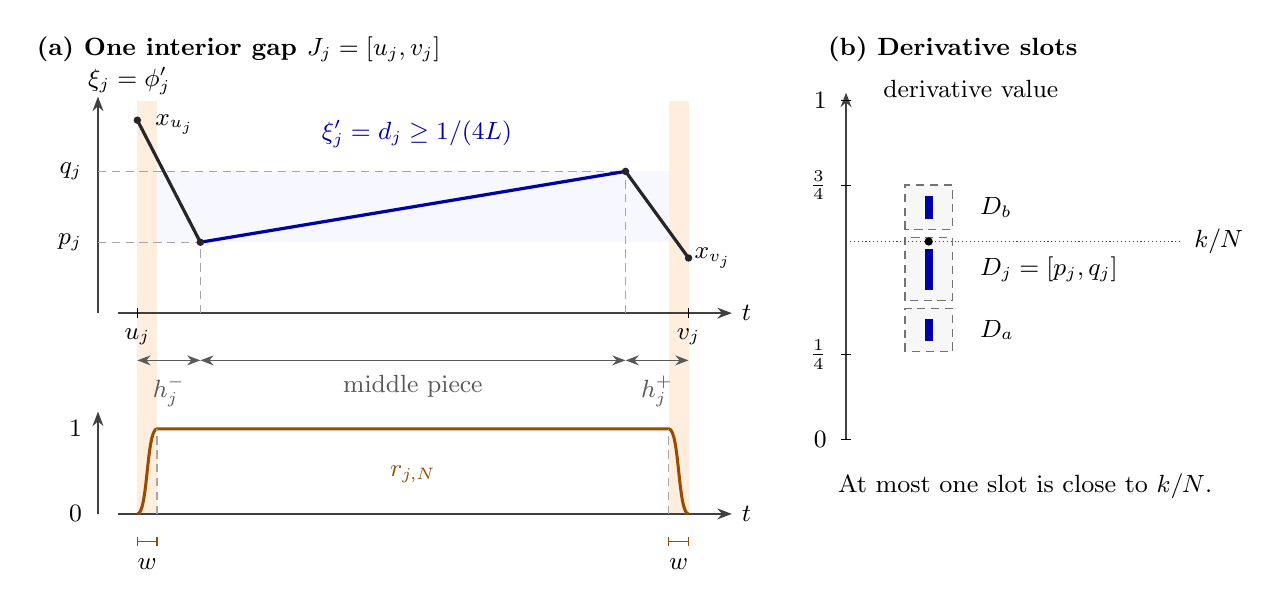
\begin{tikzpicture}[
  x=1cm,y=1cm,
  font=\small,
  >=Stealth,
  phase/.style={draw=blue!65!black,line width=1.15pt},
  taper/.style={draw=orange!60!black,line width=1.1pt},
  guide/.style={draw=black!35,densely dashed,line width=.4pt},
  axis/.style={draw=black!75,line width=.5pt,->},
  slot/.style={draw=blue!65!black,line width=3pt},
  neighborhood/.style={draw=black!55,densely dashed,fill=black!3,line width=.5pt}
]
\node[anchor=west,font=\small\bfseries] at (0,6.55)
  {(a) One interior gap $J_j=[u_j,v_j]$};
\fill[blue!3] (1.4,4.1) rectangle (8.4,5.0);
\fill[orange!13] (1.4,.65) rectangle (1.65,5.9);
\fill[orange!13] (8.15,.65) rectangle (8.4,5.9);
\draw[axis] (.9,3.2) -- (.9,5.95);
\draw[axis] (1.15,3.2) -- (8.95,3.2) node[right] {$t$};
\node[anchor=west] at (.65,6.15) {$\xi_j=\phi_j'$};
\draw[guide] (.9,4.1) -- (2.2,4.1);
\draw[guide] (.9,5.0) -- (7.6,5.0);
\node[anchor=east] at (.82,4.1) {$p_j$};
\node[anchor=east] at (.82,5.0) {$q_j$};
\draw[guide] (2.2,3.2) -- (2.2,4.1);
\draw[guide] (7.6,3.2) -- (7.6,5.0);
\draw[black!85,line width=1.15pt] (1.4,5.65) -- (2.2,4.1);
\draw[phase] (2.2,4.1) -- (7.6,5.0);
\draw[black!85,line width=1.15pt] (7.6,5.0) -- (8.4,3.9);
\foreach \x/\y in {1.4/5.65,2.2/4.1,7.6/5.0,8.4/3.9}
  \fill[black!85] (\x,\y) circle (1.35pt);
\node[anchor=west,inner sep=2pt] at (1.55,5.6) {$x_{u_j}$};
\node[anchor=west,inner sep=2pt] at (8.4,3.9) {$x_{v_j}$};
\node[anchor=south,text=blue!65!black] at (4.95,5.18)
  {$\xi_j'=d_j\ge 1/(4L)$};
\draw (1.4,3.26) -- (1.4,3.14);
\draw (8.4,3.26) -- (8.4,3.14);
\node[anchor=north] at (1.4,3.13) {$u_j$};
\node[anchor=north] at (8.4,3.13) {$v_j$};
\draw[<->,black!65] (1.4,2.6) -- (2.2,2.6)
  node[midway,below=2pt] {$h_j^-$};
\draw[<->,black!65] (2.2,2.6) -- (7.6,2.6)
  node[midway,below=2pt] {middle piece};
\draw[<->,black!65] (7.6,2.6) -- (8.4,2.6)
  node[midway,below=2pt] {$h_j^+$};
\draw[axis] (.9,.65) -- (.9,1.95);
\draw[axis] (1.15,.65) -- (8.95,.65) node[right] {$t$};
\node[anchor=east] at (.82,1.73) {$1$};
\node[anchor=east] at (.82,.65) {$0$};
\node[text=orange!60!black] at (4.9,1.15) {$r_{j,N}$};
\draw[taper] (1.4,.65)
  .. controls (1.535,.65) and (1.515,1.73) .. (1.65,1.73)
  -- (8.15,1.73)
  .. controls (8.285,1.73) and (8.265,.65) .. (8.4,.65);
\draw[guide] (1.65,.65) -- (1.65,1.73);
\draw[guide] (8.15,.65) -- (8.15,1.73);
\draw[orange!60!black] (1.4,.30) -- (1.65,.30);
\draw[orange!60!black] (8.15,.30) -- (8.4,.30);
\foreach \x in {1.4,1.65,8.15,8.4}
  \draw[orange!60!black] (\x,.24) -- (\x,.36);
\node[anchor=north] at (1.525,.20) {$w$};
\node[anchor=north] at (8.275,.20) {$w$};
\node[anchor=west,font=\small\bfseries] at (10.05,6.55)
  {(b) Derivative slots};
\draw[axis] (10.4,1.6) -- (10.4,6.0);
\node[anchor=west] at (10.75,6.05) {derivative value};
\foreach \y/\lab in {1.6/0,2.675/{\frac14},4.825/{\frac34},5.9/1} {
  \draw (10.34,\y) -- (10.46,\y);
  \node[anchor=east] at (10.28,\y) {$\lab$};
}
\draw[neighborhood] (11.15,2.71) rectangle (11.75,3.26);
\draw[neighborhood] (11.15,3.36) rectangle (11.75,4.16);
\draw[neighborhood] (11.15,4.26) rectangle (11.75,4.825);
\draw[slot] (11.45,2.85) -- (11.45,3.12);
\draw[slot] (11.45,3.5) -- (11.45,4.02);
\draw[slot] (11.45,4.4) -- (11.45,4.685);
\node[anchor=west] at (11.98,2.985) {$D_a$};
\node[anchor=west] at (11.98,3.76) {$D_j=[p_j,q_j]$};
\node[anchor=west] at (11.98,4.5425) {$D_b$};
\draw[black!75,densely dotted] (10.4,4.11) -- (14.65,4.11);
\fill (11.45,4.11) circle (1.5pt);
\node[anchor=west] at (14.7,4.11) {$k/N$};
\node[align=center,text width=4.7cm] at (12.65,1.0)
  {At most one slot is close to $k/N$.};
\end{tikzpicture}
\caption{Schematic of the correction.  In (a), the leading phase
derivative $\xi_j=\phi_j'$ matches the prescribed endpoint values and
traverses $D_j$ on the middle piece.  The outer lengths $h_j^\pm$ are
fixed; the shaded taper strips have shrinking width $w=N^{-3/4}$,
enlarged here.  The lower curve shows the amplitude factor for an
interior gap.  In (b), the dashed neighborhoods of the slots are fixed
and disjoint.  At most one middle piece and its reflection can have a
leading phase derivative close to $k/N$; all other middle pieces are
nonstationary.}
\label{fig:gap-slots}
\end{figure}


On a gap outside its transition strips, the reverse triangle inequality
gives
\[
 |B_N+R_N|\ge A-b=\frac38.
\]
To check a transition strip at $z$, compare the phases after subtracting
their values at $z$.  Since $\phi_j'(z)=\psi_z'(z)$ and both derivatives
are Lipschitz near $z$,
\[
 \bigl|\phi_j(t)-\phi_j(z)-\psi_z(t)+\psi_z(z)\bigr|
       \le C_\delta|t-z|^2.
\]
Together with \eqref{eq:gamma-bounds} and the endpoint phase agreement,
this shows that the two phases differ, modulo an integer, by at most
\begin{equation}\label{eq:phase-strip-error}
 C_\delta(Nw^2+w)=O_\delta(N^{-1/2}).
\end{equation}
Consequently, throughout that strip,
\[
 B_N(t)+R_N(t)
 =\e\bigl(\alpha_z+N\psi_z(t)\bigr)
       \bigl(B(t)+A r_{j,N}(t)+O_\delta(N^{-1/2})\bigr).
\]
Because $B(z)=b$ and $B$ is fixed and smooth, $B(t)\ge b-O_\delta(w)$
there.  This proves the lower bound $b-o(1)$ on every strip.  Off the gaps,
$R_N=0$ and $B\ge b$, and reflection preserves all these modulus bounds.
The upper bound is simpler: on gaps $|B_N+R_N|\le b+A=5/8<K_\delta$,
and elsewhere it is at most $K_\delta$.  This proves
\eqref{eq:corrected-envelope}.

The correction now gives the required lower envelope.  The remaining
task is to show that its Fourier coefficients cost only $O(\sqrt\delta)$
on the scale $N^{-1/2}$ and that discarding frequencies outside
$\{0,\ldots,N-1\}$ changes it uniformly by $o(1)$.

\subsection{A bound for each Fourier coefficient}

Split the integral for $\widehat R_N(k)$ into the three pieces of every
gap and their reflections.  On a positive piece its contribution has
the form
\begin{equation}\label{eq:piece-integral}
 \int_I a(t)\e\bigl(N\phi(t)-kt\bigr)\,dt,
 \qquad a(t)=A r_{j,N}(t)\e\bigl(\gamma_{j,N}(t)\bigr),
 \quad \phi=\phi_j|_I.
\end{equation}
On the reflected piece we use
$\phi(t)=-\phi_j(-t)$ and
$a(t)=\overline{A r_{j,N}(-t)\e(\gamma_{j,N}(-t))}$.
In particular, the reflected phase derivative is
\begin{equation}\label{eq:reflected-derivative}
 \phi'(t)=\xi_j(-t).
\end{equation}
Thus the original and reflected middle pieces use the same slot $D_j$.
By \eqref{eq:gamma-bounds} and \eqref{eq:taper-variation}, on every piece
\begin{equation}\label{eq:amplitude-bv}
 \sup_I|a|+\int_I|a'(t)|\,dt
 \le A+2A+2\pi A=:C_1.
\end{equation}
This constant is absolute, even if a gap is very short or there are many
gaps.

We use two elementary oscillatory integral estimates.  If $\phi$ is
quadratic with $\phi''=d\ne0$, then
\begin{equation}\label{eq:quadratic-integral}
 \left|\int_I a(t)\e\bigl(N\phi(t)-kt\bigr)\,dt\right|
 \le \frac{C}{\sqrt{N|d|}}
       \left(\sup_I|a|+\int_I|a'|\right).
\end{equation}
Indeed, completing the square and scaling reduce the integral without
$a$ over any subinterval to an integral of $\e(\pm u^2/2)$, multiplied
by $(N|d|)^{-1/2}$.  Those integrals are uniformly bounded: on $[-1,1]$
use length, and on each exterior half-line integrate by parts using the
phase derivative $\pm u$.  Integration against a primitive then proves
\eqref{eq:quadratic-integral}.  We also use the first-derivative bound
\begin{equation}\label{eq:first-derivative-integral}
 \left|\int_I a(t)\e\bigl(N\phi(t)-kt\bigr)\,dt\right|
 \le \frac{C}{N\rho}
       \left(\sup_I|a|+\int_I|a'|\right)
\end{equation}
when $N\phi'-k$ is monotone and has absolute value at least $N\rho$ on
$I$.  One integration by parts proves this bound, since the total
variation of $1/(N\phi'-k)$ is at most $2/(N\rho)$.

Let $C_2$ be the absolute constant obtained by combining
\eqref{eq:amplitude-bv} with \eqref{eq:quadratic-integral}.
The outer pieces and their reflections contribute at most
\[
 \frac{2C_2\sqrt\delta}{\sqrt N}
\]
by \eqref{eq:outer-slope-budget}.  For the middle pieces choose a fixed
$\rho>0$ so that the closed $\rho$-neighborhoods of the finitely many
slots $D_j$ are disjoint.  For any $k$, at most one slot is within
distance $\rho$ of $k/N$.  On that middle piece and its reflection,
\eqref{eq:quadratic-integral} and \eqref{eq:middle-slope} give a total
bound
\[
 \frac{4C_2\sqrt L}{\sqrt N}.
\]
On all remaining middle pieces, $|N\phi'-k|\ge N\rho$, so
\eqref{eq:first-derivative-integral} bounds their total contribution
by $O_\delta(N^{-1})$, uniformly in $k$.  The number of pieces and the
separation $\rho$ enter only this last error.  We conclude that
\[
 \sqrt N\,|\widehat R_N(k)|
 \le 2C_2\sqrt\delta+4C_2\sqrt L+O_\delta(N^{-1/2}).
\]
Since $L\le10\delta$, for sufficiently large $N$ this is at most
$D\sqrt\delta$ with, for example,
$D=2C_2+4\sqrt{10}C_2+1$.  This proves
\eqref{eq:correction-coefficients} with an absolute constant.
Hermitian symmetry also gives
\[
 \overline{\widehat R_N(k)}
 =\int_\T\overline{R_N(t)}\e(kt)\,dt
 =\int_\T R_N(-t)\e(kt)\,dt
 =\widehat R_N(k).
\]

\subsection{The Fourier mass outside the coefficient interval}

Let $k<0$ or $k\ge N$, and write $T=N+|k|$.
On each piece in \eqref{eq:piece-integral}, set
\[
 V(t)=N\phi'(t)-k.
\]
The derivative containment \eqref{eq:derivative-interior}, also valid on
reflected pieces by \eqref{eq:reflected-derivative}, implies
\begin{equation}\label{eq:exterior-derivatives}
 |V(t)|\ge c_\delta T,
 \qquad |V'(t)|\le C_\delta N,
 \qquad V''(t)=0
\end{equation}
on each piece interior, after decreasing $c_\delta$ if necessary.
The scaled smooth steps and the affine phase adjustments give
\begin{equation}\label{eq:amplitude-two-derivatives}
 \sup_I|a'|\le C_\delta w^{-1},
 \qquad \int_I|a''(t)|\,dt\le C_\delta w^{-1}.
\end{equation}
For the second estimate, the term of size $w^{-2}$ from a differentiated
step is supported on a strip of length $w$; the other terms are bounded
using \eqref{eq:gamma-bounds}.  Recall also the absolute bounds on
$\sup|a|$ and $\int|a'|$ in \eqref{eq:amplitude-bv}.

One integration by parts on a piece gives
\begin{equation}\label{eq:first-ibp-tail}
 \int_I a\,\e(N\phi-kt)
 =\left[\frac{a\,\e(N\phi-kt)}{2\pi iV}\right]_{\partial I}
 -\frac1{2\pi i}\int_I(a/V)'\,\e(N\phi-kt).
\end{equation}
The boundary terms in this first integration cancel when all pieces
are summed.  At a join within a gap, the numerator is the continuous
function $R_N(t)\e(-kt)$ and the denominator agrees because $\phi_j'$
is continuous.  At transition endpoints the numerator vanishes.
At $0$, the reflected and original phase derivatives both equal $x_0$,
and the numerator has the common value $A$.  Finally, at the identified
endpoints $-1/2$ and $1/2$, both phase derivatives equal $x_{1/2}$ and
the numerator has the common value $A(-1)^k$.  Thus cancellation holds
on the full circle, including the two reflection joins.

For a second integration by parts define, on each piece,
\[
 Q=\frac{(a/V)'}{V}
   =\frac{a'}{V^2}-\frac{aV'}{V^3}.
\]
No cancellation of the new boundary terms is needed.  Using $V''=0$,
\begin{equation}\label{eq:second-ibp-algebra}
 Q'=\frac{a''}{V^2}
       -\frac{3a'V'}{V^3}
       +\frac{3a(V')^2}{V^4}.
\end{equation}
Equations \eqref{eq:exterior-derivatives} and
\eqref{eq:amplitude-two-derivatives} bound the endpoint values of $Q$ by
\[
 C_\delta\left(\frac{w^{-1}}{T^2}+\frac{N}{T^3}\right)
\]
and the integral of $|Q'|$ by
\[
 C_\delta\left(\frac{w^{-1}}{T^2}
                 +\frac{N}{T^3}+\frac{N^2}{T^4}\right).
\]
Summing over the fixed finite number of pieces in
\eqref{eq:first-ibp-tail}, and integrating its remaining integrals once
more, therefore gives
\[
 |\widehat R_N(k)|
 \le C_\delta\left(\frac{w^{-1}}{T^2}
                 +\frac{N}{T^3}+\frac{N^2}{T^4}\right)
 \le \frac{C_\delta w^{-1}}{(N+|k|)^2}.
\]
Since
$\sum_{k<0\text{ or }k\ge N}(N+|k|)^{-2}=O(N^{-1})$,
we obtain
\[
 \sum_{k<0\text{ or }k\ge N}|\widehat R_N(k)|
       \le C_\delta(Nw)^{-1}=O_\delta(N^{-1/4}),
\]
as asserted in \eqref{eq:correction-tail}.  This completes the proof
of Proposition~\ref{prop:correction}.
\hfill$\square$

In particular, the Fourier series of $R_N$ is absolutely convergent.
Its sum equals $R_N$: both are continuous and have the same Fourier
coefficients, so uniqueness of Fourier coefficients applies.  Hence
\begin{equation}\label{eq:correction-projection}
 \sup_{t\in\T}
 \left|R_N(t)-\sum_{k=0}^{N-1}\widehat R_N(k)\e(kt)\right|
       =O_\delta(N^{-1/4}).
\end{equation}
We may therefore add the correction using only the required consecutive
degrees, with a uniform error tending to zero.

\section{Rounding with a small defect mass}\label{sec:rounding}

The uniform rounding error bounds the loss in the lower modulus and the
increase in the upper modulus.  The following estimate controls that
error in terms of the total distance of the relaxed coefficients from
signs.  We give the full argument from
\cite[Section~6]{OpenAIMinimal}.  Its discrepancy input belongs to
Spencer's partial-coloring method \cite{Spencer1985}; the precise
real-vector theorem used below is due to Lovett and Meka
\cite[Theorem~4 of arXiv:1203.5747v2]{LovettMeka2015}.

\begin{lemma}[Rounding with a small defect]\label{lem:rounding}
There is an absolute constant $C$ with the following property.
Let $N\ge1$ be an integer and let
$X=(X_0,\ldots,X_{N-1})\in[-1,1]^N$.  Put
\[
 \mu(X)=\frac12\sum_{k=0}^{N-1}(1-|X_k|).
\]
Then there are signs $\varepsilon_0,\ldots,\varepsilon_{N-1}$ satisfying
\begin{equation}\label{eq:defect-rounding}
 \max_{t\in\T}\left|\sum_{k=0}^{N-1}(\varepsilon_k-X_k)\e(kt)\right|
 \le C\left(1+\sqrt{\mu(X)\log\frac{80N}{\mu(X)}}\right).
\end{equation}
The square-root term is defined to be zero when $\mu(X)=0$.
In that case one may take $\varepsilon=X$, giving zero error.
\end{lemma}

We first obtain a discrepancy estimate for arbitrary real matrices.
We then round the coefficient defects on successively coarser dyadic
grids.  At every scale a simultaneous reversal of the discrepancy signs
keeps the total defect mass from increasing.  This controls how many
coordinates can move and yields the dependence on $\mu(X)$.

\subsection{A discrepancy bound for real matrices}

\begin{lemma}\label{lem:rounding-matrix}
There is an absolute constant $C_0$ such that, for integers $1\le s\le R$
and a real matrix $B\in[-1,1]^{R\times s}$, there is a vector
$\xi\in\{-1,1\}^s$ satisfying
\[
 \norm{B\xi}_\infty\le C_0\sqrt{s\log(2R/s)}.
\]
\end{lemma}

\begin{proof}
We use the following existential consequence of the Lovett--Meka theorem
\cite[Theorem~4 of arXiv:1203.5747v2]{LovettMeka2015}.
Given vectors $v_1,\ldots,v_R\in\R^u$, a starting point
$x_0\in[-1,1]^u$, and
nonnegative numbers $c_1,\ldots,c_R$ such that
\[
 \sum_{i=1}^R\exp(-c_i^2/16)\le u/16,
\]
there exists, for every sufficiently small $\eta>0$, a point
$x\in[-1,1]^u$ with
\[
 |\langle v_i,x-x_0\rangle|\le c_i\norm{v_i}_2
 \quad(1\le i\le R),
 \qquad
 |x_k|\ge1-\eta\quad\text{for at least }u/2\text{ coordinates }k.
\]
The cited theorem finds such a point with positive probability; we use
only its existence assertion.  Letting $\eta$ tend to zero and taking a
convergent subsequence in the compact cube gives a
point with at least $\lceil u/2\rceil$ coordinates equal to signs and the
same discrepancy bounds.  Indeed, there are only finitely many choices
of these coordinates, and all the displayed inequalities are closed
under limits.

Start at zero in $[-1,1]^s$.  At a stage with $u$ coordinates not yet
equal to signs, restrict the rows of $B$ to those coordinates, take their
current values as $x_0$, and choose
\[
 c_i=4\sqrt{\log(16R/u)}\qquad(1\le i\le R).
\]
The threshold sum is exactly $u/16$, and every restricted row has
Euclidean norm at most $\sqrt u$.  Thus this step changes each row sum
by at most $4\sqrt{u\log(16R/u)}$ and fixes at least half the remaining
coordinates.  Leave the fixed coordinates unchanged and repeat.
Zero rows impose no restriction.  The process terminates with a sign
vector.

If $u_h$ is the number of remaining coordinates before step $h$, starting
with $h=0$, then $u_h\le2^{-h}s$.  The function
$u\log(16R/u)$ is increasing for $0<u\le R$.  With
$L=\log(16R/s)\ge\log16$, the sum of the row errors is therefore at most
\[
 \begin{aligned}
 4\sum_h\sqrt{u_h\log(16R/u_h)}
 &\le4\sqrt{sL}\sum_{h=0}^{\infty}2^{-h/2}
       \sqrt{1+\frac{h\log2}{L}}\\
 &\le4\sqrt{sL}\sum_{h=0}^{\infty}2^{-h/2}\sqrt{1+h/4}.
 \end{aligned}
\]
The last series converges, and $\log(16R/s)\le4\log(2R/s)$ for $s\le R$.
This proves the lemma with an absolute constant, including when $s=R$.
\end{proof}

\subsection{Dyadic rounding and the Fourier error}

Apply the matrix estimate to real and imaginary Fourier evaluations on
a grid of $20N$ points.  After dyadic rounding, a derivative bound for
the error polynomial will transfer the estimate to the whole circle.

\begin{proof}[Proof of Lemma~\ref{lem:rounding}]
Let $X=(X_0,\ldots,X_{N-1})\in[-1,1]^N$ and
$\mu=\frac12\sum_k(1-|X_k|)$.  If $\mu=0$, every $X_k$ is already a
sign, and we take $\varepsilon_k=X_k$.  Suppose henceforth that
$0<\mu\le N/2$.  Set
\[
 \sigma_k=\begin{cases}1,&X_k\ge0,\\-1,&X_k<0,\end{cases}
 \qquad p_k=\frac{1-|X_k|}{2}.
\]
Then $X_k=\sigma_k(1-2p_k)$, $0\le p_k\le1/2$, and
$\sum_kp_k=\mu$.  In particular, this definition includes $X_k=0$.

Put $M=20N$ and $R=2M=40N$.  For the grid points
$t_\ell=\ell/M$, $0\le\ell<M$, define the real $R\times N$ matrix $A$ by
\[
 A_{2\ell,k}=\sigma_k\cos(2\pi kt_\ell),\qquad
 A_{2\ell+1,k}=\sigma_k\sin(2\pi kt_\ell)
 \quad(0\le k<N).
\]
Its entries belong to $[-1,1]$, and every selection of its columns has
at most $N\le R$ columns.

Choose an integer $J\ge1$ with $N2^{-J}\le1$, and first round down:
\[
 p^{(J)}_k=2^{-J}\lfloor2^Jp_k\rfloor.
\]
This does not increase the mass, and
\begin{equation}\label{eq:rounding-initial}
 \norm{A(p^{(J)}-p)}_\infty
 \le\sum_k|p^{(J)}_k-p_k|\le N2^{-J}\le1.
\end{equation}
We next construct $p^{(j-1)}$ from $p^{(j)}$, for $j=J,J-1,\ldots,1$.
Intermediate entries may exceed $1/2$, but it is enough to keep them in
$[0,1]$, whose endpoints encode the two choices of final sign.  We
preserve the two properties
\[
 p^{(j)}\in([0,1]\cap2^{-j}\Z)^N,
 \qquad \sum_kp^{(j)}_k\le\mu.
\]
Let $S_j$ be the set of coordinates for which $2^jp^{(j)}_k$ is odd,
and let $s_j=|S_j|$.  If $s_j=0$, no change is needed.  Otherwise apply
Lemma~\ref{lem:rounding-matrix} to the columns indexed by $S_j$, obtaining
signs $\xi_k$.  Replace all these signs by their negatives if necessary
so that $\sum_{k\in S_j}\xi_k\le0$, and define
\[
 p^{(j-1)}_k=
 \begin{cases}
 p^{(j)}_k+2^{-j}\xi_k,&k\in S_j,\\
 p^{(j)}_k,&k\notin S_j.
 \end{cases}
\]
An odd integer in $[0,2^j]$ lies between $1$ and $2^j-1$; adding either
sign therefore gives an even integer still in $[0,2^j]$.  Thus the
new vector belongs to $([0,1]\cap2^{-(j-1)}\Z)^N$.  Its mass does not
increase, and the simultaneous sign reversal has left the discrepancy
unchanged.  The step error is consequently at most
\begin{equation}\label{eq:rounding-step}
 \norm{A(p^{(j-1)}-p^{(j)})}_\infty
 \le C_0\,2^{-j}\sqrt{s_j\log(80N/s_j)}
 \qquad(s_j>0).
\end{equation}

Every coordinate in $S_j$ is at least $2^{-j}$, so the mass bound gives
\[
 s_j\le\min(N,2^j\mu).
\]
This is where the total defect enters the estimate.  Put
$U_j=2^j\mu$ and $L_\mu=\log(80N/\mu)$.  The function
$f(s)=s\log(80N/s)$ is increasing on $(0,N]$.  If $U_j\le N$, then
\[
 f(s_j)\le f(U_j)
 =U_j\log(80N/U_j)\le U_jL_\mu.
\]
If $U_j>N$, then, using $\mu\le N/2$,
\[
 f(s_j)\le N\log80\le U_jL_\mu.
\]
These estimates apply at every nonempty stage.  Summing
\eqref{eq:rounding-step} and \eqref{eq:rounding-initial} therefore gives,
for $p'=p^{(0)}\in\{0,1\}^N$,
\begin{equation}\label{eq:rounding-matrix-error}
 \begin{aligned}
 \norm{A(p'-p)}_\infty
 &\le1+C_0\sqrt{\mu L_\mu}\sum_{j=1}^{\infty}2^{-j/2}\\
 &=1+\frac{C_0}{\sqrt2-1}\sqrt{\mu\log(80N/\mu)}.
 \end{aligned}
\end{equation}
Empty stages contribute zero, without invoking the discrepancy bound
with no columns.

Now set $\varepsilon_k=\sigma_k(1-2p'_k)\in\{-1,1\}$ and define the
error polynomial
\[
 Q(z)=\sum_{k=0}^{N-1}(\varepsilon_k-X_k)z^k
     =-2\sum_{k=0}^{N-1}\sigma_k(p'_k-p_k)z^k.
\]
By the definition of $A$, the real and imaginary parts of
$Q(\e(t_\ell))$ each have absolute value at most
$2\norm{A(p'-p)}_\infty$.  Hence
\begin{equation}\label{eq:rounding-grid}
 G:=\max_{0\le\ell<M}|Q(\e(t_\ell))|
 \le2\sqrt2\,\norm{A(p'-p)}_\infty.
\end{equation}
It remains to pass from this grid bound to the whole circle.  We apply
this step only to $Q$, the rounding error.

Write $S=\max_{|z|=1}|Q(z)|$.  If $Q=0$, there is nothing to prove.
Otherwise let $d\le N-1$ be its degree.  Applying the maximum principle
to $Q$ on the unit disk and to the reversed polynomial $z^dQ(1/z)$ gives
\[
 |Q(z)|\le S\max(1,|z|^d),
 \qquad
 \max_{|z|\le1+1/N}|Q(z)|\le \exp(1)S.
\]
Cauchy's estimate on the disk of radius $1/N$ centered at a point of
the unit circle yields $|Q'(z)|\le\exp(1)NS$ there.  Consequently
\[
 \left|\frac{d}{dt}Q(\e(t))\right|
 \le2\pi\exp(1)NS.
\]
Every point of $\T$ has circular distance at most $1/(2M)$ from the
grid.  Integrating this derivative along the shorter arc gives
\[
 S\le G+\frac{\pi\exp(1)}{20}S,
 \qquad
 S\le\frac{G}{1-\pi\exp(1)/20}.
\]
The denominator is positive.  Combining this inequality with
\eqref{eq:rounding-grid} and \eqref{eq:rounding-matrix-error} proves
Lemma~\ref{lem:rounding}, with an absolute constant.  The same argument
covers $N=1$, when the error polynomial is constant.
\end{proof}

\section{Proof of the main theorem}\label{sec:completion}
We now combine the construction with the rounding estimate. The order of
the choices is important: the accuracy parameter fixes all auxiliary data,
and only then does the length tend to infinity.

\begin{proof}[Proof of Theorem~\ref{thm:main}]
Let $b=1/8$ and let $D>0$ be the absolute constant in
Proposition~\ref{prop:correction}.
For a fixed sufficiently small $\delta>0$, take the real coefficients
$Y_{N,k}$ and the functions $B_N$ from Proposition~\ref{prop:starting},
and the correction $R_N$ from Proposition~\ref{prop:correction}.
All estimates below hold for every sufficiently large integer $N$.
Put
\[
 s_\delta=D\sqrt\delta,\qquad S_\delta=1+s_\delta,
 \qquad
 X_{N,k}=\frac{Y_{N,k}+\sqrt N\,\widehat R_N(k)}{S_\delta}
 \quad(0\le k<N).
\]
Conjugate symmetry of $R_N$ makes $\widehat R_N(k)$ real. Since
$|Y_{N,k}|\le1$ and $\sqrt N|\widehat R_N(k)|\le s_\delta$,
the vector $X_N$ belongs to $[-1,1]^N$.
The uniform approximation in Proposition~\ref{prop:starting} and the
exterior Fourier-tail estimate in Proposition~\ref{prop:correction} give
\begin{equation}\label{eq:completion-profile}
 U_{X_N}(t)=\frac{B_N(t)+R_N(t)}{S_\delta}+o(1)
 \qquad\text{uniformly for }t\in\T.
\end{equation}
Consequently,
\begin{equation}\label{eq:completion-envelope}
 \min_{t\in\T}|U_{X_N}(t)|\ge\frac b{S_\delta}-o(1),
 \qquad
 \norm{U_{X_N}}_\infty\le K_\delta+o(1).
\end{equation}
In the second inequality we used $S_\delta\ge1$.

The same coefficient bound controls the cost of rounding. Directly,
\[
 |X_{N,k}-Y_{N,k}|
 =\frac{|\sqrt N\,\widehat R_N(k)-s_\delta Y_{N,k}|}{S_\delta}
 \le2s_\delta.
\]
Both coefficients lie in $[-1,1]$, so
$|X_{N,k}^2-Y_{N,k}^2|\le4s_\delta$.
Using the mean-square estimate from Proposition~\ref{prop:starting} and
$1-|x|\le1-x^2$ for $|x|\le1$, we obtain
\begin{equation}\label{eq:completion-defect}
 \frac{\mu(X_N)}N
 \le\frac1{2N}\sum_{k=0}^{N-1}(1-X_{N,k}^2)
 \le4\delta+2D\sqrt\delta=:q_\delta.
\end{equation}
Choose $\delta$ small enough that $q_\delta<1/2$.
The function $q\mapsto q\log(80/q)$ is increasing on $(0,1/2]$.
Lemma~\ref{lem:rounding} therefore supplies signs
$\varepsilon_0,\ldots,\varepsilon_{N-1}$ with
\begin{equation}\label{eq:completion-rounding}
 \norm{U_\varepsilon-U_{X_N}}_\infty
 \le \frac C{\sqrt N}
       +C\sqrt{q_\delta\log(80/q_\delta)}.
\end{equation}
If $\mu(X_N)=0$, we instead take $\varepsilon_k=X_{N,k}$, so this bound
also covers that case.

Fix $c=1/16$ once and for all. As $\delta\downarrow0$,
\[
 \frac b{S_\delta}
       -C\sqrt{q_\delta\log(80/q_\delta)}\longrightarrow\frac18,
 \qquad
 K_\delta+C\sqrt{q_\delta\log(80/q_\delta)}\longrightarrow1.
\]
For any prescribed $\eta>0$, first choose $\delta$ so small that the
first expression is strictly larger than $c$ and the second is strictly
smaller than $1+\eta$. Fix every construction datum associated with this
$\delta$. We may then choose $N_0$ so that for every $N\ge N_0$ all preceding
estimates hold and the errors in \eqref{eq:completion-envelope} and
\eqref{eq:completion-rounding} are smaller than these strict margins.
It follows that
\[
 c\le|U_\varepsilon(t)|\le1+\eta\qquad(t\in\T).
\]
Multiplication by $\sqrt N$ gives the asserted polynomial. Rounding assigns
a real sign to each of the consecutive indices $0,\ldots,N-1$; all
estimates include $t=0$ and $t=1/2$ and hold through every sufficiently
large integer length.
\end{proof}

\bibliographystyle{plain}
\bibliography{refs}
\end{document}
